% Prepared for submission to: Computational Intelligence (Wiley)
% Publisher: Wiley
% Submission portal: https://wiley.atyponrex.com/journal/COIN (Wiley Author Services)
% Modern pdfTeX already runs in etex-extended mode, so WileyNJD-v2.cls's
% \usepackage{etex}; \reserveinserts{28} call finds etex.sty a no-op and
% \reserveinserts undefined. Pre-define it as a no-op to avoid a fatal error.
\providecommand{\reserveinserts}[1]{}
\documentclass[AMA,STIX1COL,]{WileyNJD-v2}

\usepackage{amssymb}
\usepackage{array}
\usepackage{pgfplots}
\usepackage{tikz}

\pgfplotsset{compat=1.18}
\usetikzlibrary{arrows.meta,shapes,positioning,calc}
\usepgfplotslibrary{colorbrewer}
\usepgfplotslibrary{patchplots}

\lstset{
  basicstyle=\tiny\ttfamily,
  breaklines=true,
  frame=tb,
  language=Python,
  keywordstyle=\color{blue!70},
  commentstyle=\color{gray},
  stringstyle=\color{orange!80!black},
  numbers=left,
  numberstyle=\tiny\color{gray},
  numbersep=4pt,
  xleftmargin=8pt
}

\articletype{Research Article}

\raggedbottom

\begin{document}

\title{DeepCardio-RAG: A Multi-Modal Retrieval-Augmented Generation
Framework for AI-Assisted Cardiac Diagnosis Integrating ECG,
Echocardiography, Heart Sound, Ventricular Arrhythmia, and
Self-Reported Arthritis Risk}

\author[1]{N. Rama Rao}
\author[2]{Durgesh Nandan}
\author[3]{S. Satyanarayana}
\author[4]{N. Soumya}

\authormark{Rama Rao \emph{et al.}}

\address[1]{\orgdiv{Department of Artificial Intelligence}, \orgname{SR University}, \orgaddress{Warangal, Telangana, India}; \orgname{Koneru Lakshmaiah Education Foundation}, \orgaddress{Hyderabad, Telangana, India}}
\address[2]{\orgdiv{School of Computer Science and Artificial Intelligence}, \orgname{SR University}, \orgaddress{Warangal, Telangana, India}}
\address[3]{\orgdiv{Department of Artificial Intelligence and Data Science}, \orgname{Sanjivani University}, \orgaddress{Kopargaon, Maharashtra, India}}
\address[4]{\orgname{Bhaskar Medical College}, \orgaddress{Moinabad, Hyderabad, Telangana, India}}

\corres{*N. Rama Rao, Department of Artificial Intelligence, SR University, Warangal, Telangana, India. Tel.: +91-9951987846. \email{ramarao.n@klh.edu.in}}

\abstract{Cardiovascular diseases account for 17.9~million deaths annually, yet
specialist cardiologists remain scarce in low- and middle-income
countries. This paper presents \textbf{DeepCardio-RAG}, a multi-modal
artificial-intelligence platform integrating six deep-learning modules:
an ECG Transformer with Mixture-of-Experts~(MoE) encoder for
arrhythmia classification, a 3D-CNN for left-ventricular ejection
fraction estimation, a Mel-spectrogram CNN for cardiac murmur detection,
a 1D-CNN for ventricular arrhythmia detection, and two TabularBERT-MoE
models for heart-disease and self-reported arthritis risk
stratification. We note at the outset that the arthritis target is
NHANES MCQ160A, self-reported doctor-diagnosed arthritis of any type
--- predominantly osteoarthritis --- and not serologically defined
rheumatoid arthritis.
All six modules operate under a unified Retrieval-Augmented
Generation~(RAG) pipeline backed by a Milvus vector store; a GPT-2
decoder conditioned on retrieved clinical guidelines synthesises
dual-format diagnostic report drafts. The CardioFusion module fuses
modality-specific outputs into a 100-point unified cardiac risk score.
We report the evidential position explicitly. \textbf{Five of the six
deep modules are independently trained} on public benchmarks and
evaluated on held-out data or by repeated cross-validation with
confidence intervals: flagship ECG (PTB-XL, AUC~0.801), ECG arrhythmia
(MIT-BIH, 0.928), CardioFusion ECG path (0.838), murmur detection
(CirCor, Present-vs-Absent AUC~0.761), ventricular arrhythmia (VFDB,
recording-level CV AUC~0.919), and heart-disease risk (deduplicated
UCI Cleveland, CV AUC~0.872). The \textbf{echocardiography module
remains untrained} for want of EchoNet-Dynamic access and its outputs
are suppressed rather than scored, and \textbf{report-generation
quality is not evaluated} in this work. No module matches its published
benchmark, and on the Cleveland cohort a plain logistic regression
outperforms our deep classifier. The system has not been validated for
clinical deployment and issues no treatment directives.}

\keywords{Multi-modal cardiac AI; Retrieval-Augmented Generation;
ECG arrhythmia classification; Mixture of Experts;
Self-reported arthritis risk stratification}

\maketitle

%===================================================================
\section{Introduction}
\label{sec:intro}
%===================================================================

Cardiovascular disease constitutes the single largest cause of death
globally. The World Health Organization estimates that
17.9~million lives are lost annually to CVDs, representing 32\% of all
global deaths~\cite{who2021}. This burden falls disproportionately on
low- and middle-income countries~(LMICs), where cardiologist density
can be as low as one specialist per 200\,000~inhabitants~\cite{watkins2018}.
Electrocardiography~(ECG), echocardiography, and phonocardiography
remain the primary non-invasive diagnostic modalities; however,
accurate interpretation demands years of specialist training and
remains largely inaccessible in rural and resource-constrained settings.

Artificial intelligence~(AI) offers a transformative opportunity.
Broad reviews of AI in medicine~\cite{topol2019,rajpurkar2022} and of
deep learning in healthcare specifically~\cite{esteva2019}, together with
surveys of deep learning in medical image
analysis~\cite{litjens2017,shen2017} and the standard treatment of the
underlying methods~\cite{goodfellow2016}, document
rapid gains across diagnostic specialties, with cardiovascular medicine
identified early as a leading application area~\cite{krittanawong2017}.
Deep learning~(DL) models trained on large ECG corpora have demonstrated
cardiologist-level accuracy for arrhythmia detection. Hannun
\emph{et~al.}~\cite{hannun2019} reported a 12-rhythm classification
model achieving a mean AUC-ROC of~0.97 on a single-lead ECG dataset,
surpassing the average board-certified cardiologist on six of twelve
rhythms. Rajpurkar \emph{et~al.}~\cite{rajpurkar2017} demonstrated
that convolutional neural networks trained on 64\,121~ECG recordings
outperformed cardiologists on arrhythmia classification. Ouyang
\emph{et~al.}~\cite{ouyang2020} introduced EchoNet-Dynamic, a 3D-CNN
that estimates LVEF from echocardiographic video with a mean absolute
error of~4.1\%, setting the standard for automated ejection fraction
assessment.

Despite these advances, standalone DL models suffer from a critical
limitation: hallucination and lack of evidence grounding~\cite{ji2023}.
Language models tasked with generating clinical narratives frequently
produce factually incorrect statements---a phenomenon with serious
patient-safety consequences. Retrieval-Augmented Generation~(RAG),
introduced by Lewis \emph{et~al.}~\cite{lewis2020}, addresses this by
conditioning generation on retrieved, verifiable knowledge documents.
Applied to clinical report writing, RAG can substantially reduce
hallucination while maintaining the fluency required for physician
consumption~\cite{chatdoctor2023}. Med-PaLM~\cite{singhal2023} and
GPT-4~\cite{nori2023} have demonstrated expert-level performance on
medical question answering, yet both still hallucinate clinical details
that retrieval-augmented grounding can significantly curtail.

Existing systems address cardiac diagnosis modality by modality: some
focus solely on ECG~\cite{hannun2019,rajpurkar2017,ribeiro2020},
others on echocardiography~\cite{ouyang2020,zhang2018,madani2018}, and
a smaller set on heart sounds~\cite{clifford2016,potes2016}.
Furthermore, comorbidity screening for arthritis is virtually absent
from published cardiac AI pipelines. The cardiovascular case is
clearest for rheumatoid arthritis, which carries a two-fold elevated
cardiovascular risk~\cite{avinazubieta2008}; osteoarthritis, the
dominant form in general-population survey data, is associated with
cardiovascular disease largely through shared risk factors such as
obesity, physical inactivity and age rather than through the systemic
inflammation that drives RA risk. Our module addresses the
general-population case and we do not transfer the RA-specific
comorbidity argument to it. No publicly reported system integrates all major
non-invasive cardiac modalities under a single RAG-augmented reporting
framework with a unified risk score and dual-format report generation.

\subsection{Key Contributions of This Study}

The principal contributions of this work are summarised as follows:

\begin{itemize}
  \item We present \textbf{DeepCardio-RAG}, a research prototype
        integrating six cardiac/comorbidity AI modules (ECG,
        echocardiography, heart sound, ventricular arrhythmia, heart
        disease, and arthritis) under a unified RAG pipeline with a
        shared Milvus vector store.
  \item We design a \textbf{Milvus-backed vector retrieval system}
        (768-dim Sentence-BERT embeddings, $L_2$ distance, FAISS
        fallback) with a prototype clinical guidelines corpus of
        67~chunks, enabling sub-second RAG retrieval in a working
        deployment.
  \item We propose the \textbf{CardioFusion scoring algorithm} that
        fuses modality-specific probability vectors into an
        interpretable 100-point unified cardiac risk score.
  \item We implement a \textbf{hybrid stacking ensemble} for arthritis
        risk classification (TabularBERT-MoE + GBM + RF + ExtraTrees
        $\rightarrow$ LogReg meta-learner), evaluated on a
        stratified held-out test set from the NHANES dataset~(5,756~records).
  \item We deliver a \textbf{fully working end-to-end prototype} with
        a React dashboard, FastAPI backend, dual-format PDF generation,
        and LangGraph multi-agent diagnostic orchestration.
  \item We explicitly discuss \textbf{current limitations}, including
        the use of random encoder weights, small dataset sizes, and the
        absence of prospective clinical validation, establishing a clear
        roadmap for future work.
\end{itemize}

%===================================================================
\section{Related Work}
\label{sec:related}
%===================================================================

\subsection{ECG Arrhythmia Classification}

Hannun \emph{et~al.}~\cite{hannun2019} demonstrated that a deep
residual CNN trained on 91\,232~single-lead ECG recordings classified
12~rhythms at cardiologist-level accuracy. Rajpurkar
\emph{et~al.}~\cite{rajpurkar2017} employed a 34-layer ResNet and
reported superiority over individual cardiologists on inter-rater
metrics. Ribeiro \emph{et~al.}~\cite{ribeiro2020} extended this to
12-lead analysis with 1.6~million records, achieving an $F_1$-score
above~0.80 for six abnormalities. Natarajan
\emph{et~al.}~\cite{natarajan2020} combined wide CNNs with multi-head
self-attention for 12-lead ECG classification. Baloglu
\emph{et~al.}~\cite{baloglu2019} applied a deep CNN to multi-lead ECG
for myocardial-infarction detection, the diagnostic superclass our
flagship encoder finds hardest~(per-class AUC~0.782). Sun
\emph{et~al.}~\cite{sun2024} combined ECG and phonocardiogram
(PCG) signals in a multi-modal deep-coding model, reporting
complementary diagnostic information across modalities. Strodthoff
\emph{et~al.}~\cite{strodthoff2021} benchmarked deep learning models
on PTB-XL, demonstrating that CNN ensembles achieve macro-AUC of~0.925.

\subsection{Echocardiography and LVEF Estimation}

Ouyang \emph{et~al.}~\cite{ouyang2020} introduced EchoNet-Dynamic,
reporting MAE of~4.1\% for LVEF estimation. Zhang
\emph{et~al.}~\cite{zhang2018} used a fully convolutional network for
left-ventricle segmentation, achieving Dice coefficient of~0.95 on the
CAMUS dataset~\cite{leclerc2019}. Madani \emph{et~al.}~\cite{madani2018} demonstrated
real-time echocardiography view classification at 94.4\% accuracy.
Dezaki \emph{et~al.}~\cite{dezaki2019} proposed a recurrent network
for cardiac phase detection in 3D echocardiography. Asch
\emph{et~al.}~\cite{asch2019} demonstrated automated 3D
echocardiography analysis comparable to manual expert measurements.

\subsection{Heart Sound Analysis}

The 2016 PhysioNet/CinC Challenge~\cite{clifford2016} formalised
benchmark evaluation using 3\,240~heart sound recordings; the winning
system achieved mean sensitivity~0.86. Potes \emph{et~al.}~\cite{potes2016}
combined AdaBoost and a CNN, achieving AUC~0.86. Acharya
\emph{et~al.}~\cite{acharya2017} applied a deep CNN directly to heart
sound recordings, an approach close to the Mel-spectrogram CNN adopted
here. The 2022~CirCor
DigiScope challenge~\cite{oliveira2022} extended this with
5\,272~recordings; the best-performing system achieved outcome
metric~0.789. Kay \emph{et~al.}~\cite{kay2020} applied convolutional
recurrent networks to heart sound segmentation. Deng
\emph{et~al.}~\cite{deng2020} introduced contrastive learning for
heart sound representations.

\subsection{Ventricular Arrhythmia Detection}

Acharya \emph{et~al.}~\cite{acharya2018} applied a 13-layer 1D-CNN
to MIT-BIH VFDB recordings, achieving 98.7\% accuracy for VF/VT
discrimination. Dang \emph{et~al.}~\cite{dang2019} achieved 99.1\%
sensitivity on the same corpus. Pourbabaee
\emph{et~al.}~\cite{pourbabaee2018} achieved 99.3\% for VF detection.
Fallet \emph{et~al.}~\cite{fallet2015} combined signal quality index
assessment with SVM for robust detection under clinical noise. Shaik
\emph{et~al.}~\cite{shaik2021} achieved 98.2\% accuracy including
flutter classification.

\subsection{Clinical Tabular Data and Heart Disease Risk}

Shah \emph{et~al.}~\cite{shah2020} demonstrated gradient-boosted trees
achieving AUC-ROC of~0.81--0.85 on the Cleveland and Framingham Heart
datasets. TabTransformer~\cite{huang2020} outperformed tree-based
methods by treating each feature as a token. MoE
architectures~\cite{shazeer2017} enable parameter-efficient multi-task
learning. Weng \emph{et~al.}~\cite{weng2017} found neural networks
superior in cardiovascular risk prediction~(sensitivity 0.76,
specificity~0.71).

\subsection{Arthritis and Cardiovascular Comorbidity}

RA carries a two-fold elevated cardiovascular
risk~\cite{avinazubieta2008}. ACR/EULAR 2010 criteria~\cite{aletaha2010}
score joint involvement, serology, acute-phase reactants, and symptom
duration. ML-based RA risk prediction from blood panels has been
demonstrated with AUC-ROC of~0.88--0.93~\cite{tian2020}. England
\emph{et~al.}~\cite{england2018} showed that routine blood tests
contain sufficient information for preliminary RA screening. Ziegler
\emph{et~al.}~\cite{ziegler2010} quantified cardiovascular risk
attributable to RA in a longitudinal cohort of 4\,000~patients.

These results describe \emph{serologically defined RA} and are cited as
context, not as a benchmark for our module. Our target is NHANES
MCQ160A --- self-reported, doctor-diagnosed arthritis of any type in a
household survey, a population dominated by osteoarthritis. Excluding
the skip-pattern variable MCQ195 was necessary to remove target
leakage, but its consequence is that the module cannot identify RA
specifically. The tasks therefore differ, and numerical comparison
against the 0.88--0.93 RA figures is not like-for-like; we report it
only to situate the work. Establishing the RA-specific claim would
require a cohort with serological labels, which we identify as required
future work in Section~\ref{sec:limitations}.

\subsection{Retrieval-Augmented Generation in Clinical NLP}

RAG~\cite{lewis2020} conditions generation on retrieved passages,
substantially reducing hallucination~\cite{ji2023}.
Domain-adapted encoders such as BioBERT~\cite{lee2020biobert} showed
that pre-training on biomedical corpora improves downstream clinical
text tasks --- a route this prototype does not take, since its decoder
is general-domain GPT-2.
ChatDoctor~\cite{chatdoctor2023} demonstrated improved factual accuracy
through RAG augmentation of LLaMA. Med-PaLM~\cite{singhal2023} achieved
expert-level performance on MedQA. Shi \emph{et~al.}~\cite{shi2023}
showed retrieval plug-ins improve LLM perplexity by~6.3~points on
medical corpora. Lester \emph{et~al.}~\cite{lester2021} demonstrated
that soft-prompt injection outperforms hard-prompt concatenation for
controlled generation.

\subsection{Summary of Selected Studies}

Table~\ref{tab:related_summary} presents a summary of representative
prior studies in cardiac and comorbidity AI, their key findings, and
identified shortcomings.

\begin{table*}[!ht]
\caption{Summary of selected cardiac AI studies, key findings, and limitations.}
\label{tab:related_summary}
\centering
\renewcommand{\arraystretch}{1.15}
\begin{tabular}{c>{\raggedright\arraybackslash}p{2.8cm}>{\raggedright\arraybackslash}p{4.5cm}>{\raggedright\arraybackslash}p{4.5cm}}
\toprule
\textbf{S.\,No.} & \textbf{Author name \& year} & \textbf{Findings} & \textbf{Shortcomings}\\
\midrule
1 & Hannun et~al.\ (2019)~\cite{hannun2019}
  & 12-rhythm ECG classification at cardiologist-level accuracy (AUC 0.97); single-lead
  & Single-lead only; not multimodal; no report generation\\
2 & Rajpurkar et~al.\ (2017)~\cite{rajpurkar2017}
  & 34-layer ResNet outperforms cardiologists on arrhythmia classification; 64,121 recordings
  & Single-lead; no tabular comorbidity screening\\
3 & Ribeiro et~al.\ (2020)~\cite{ribeiro2020}
  & 12-lead $F_1{>}0.80$ for six abnormalities; 1.6M records
  & No RAG report generation; single modality\\
4 & Ouyang et~al.\ (2020)~\cite{ouyang2020}
  & EchoNet-Dynamic; LVEF MAE 4.1\%; 10,030 echo videos
  & Echocardiography only; no cross-modal fusion\\
5 & Clifford et~al.\ (2016)~\cite{clifford2016}
  & PhysioNet/CinC Challenge; mean sensitivity 0.86 on 3,240 recordings
  & Heart sound only; no clinical report synthesis\\
6 & Acharya et~al.\ (2018)~\cite{acharya2018}
  & 13-layer 1D-CNN; 98.7\% accuracy for VF/VT on MIT-BIH VFDB
  & VF/VT detection only; no unified cardiac pipeline\\
7 & Shah et~al.\ (2020)~\cite{shah2020}
  & GBT; AUC-ROC 0.81--0.85 on Cleveland/Framingham heart disease datasets
  & Tabular only; no signal modalities\\
8 & Lewis et~al.\ (2020)~\cite{lewis2020}
  & Introduced RAG; reduces hallucination in open-domain NLP
  & General NLP; not applied to cardiac signals\\
9 & Singhal et~al.\ (2023)~\cite{singhal2023}
  & Med-PaLM; expert-level medical QA; strong multimodal reasoning
  & No dedicated cardiac signal encoders; general-purpose\\
10 & Tian et~al.\ (2020)~\cite{tian2020}
   & ML-based RA risk prediction from blood panels; AUC-ROC 0.88--0.93
   & RA only; not integrated with cardiac pipeline\\
\midrule
\multicolumn{4}{l}{\textbf{Proposed}} \\
 & DeepCardio-RAG (this work)
  & Six-modality cardiac + arthritis AI; Milvus RAG; CardioFusion unified risk score;
    dual-format PDF; end-to-end prototype
  & Random encoder weights; single-country NHANES survey population; no prospective clinical validation\\
\bottomrule
\end{tabular}
\end{table*}

\subsection{Research Gaps}

No published system integrates all major non-invasive cardiac
modalities under a single framework. RAG has not been applied to
multi-modal cardiac report generation with empirically measured
hallucination reduction. Unified interpretable risk scores fusing
heterogeneous modality outputs and dual-format report generation from a
single AI inference run have not been demonstrated. DeepCardio-RAG
directly addresses all four gaps.

%===================================================================
\section{Methodology}
\label{sec:methodology}
%===================================================================

\subsection{System Architecture Overview}

Figure~\ref{fig:architecture} illustrates the end-to-end DeepCardio-RAG
architecture. Patient data arrives through six modality-specific input
channels. Each channel is processed by a dedicated deep-learning
encoder producing a fixed-dimension embedding and a structured
prediction. These predictions feed two parallel pipelines: (1)~the
\textbf{CardioFusion scorer}, which computes a unified 100-point
cardiac risk index, and (2)~the \textbf{RAG report generator}, which
retrieves evidence-aligned guidelines from Milvus and synthesises
clinical and patient-facing reports through a GPT-2 decoder with
soft-prompt injection.

\begin{figure}[!t]
\centering
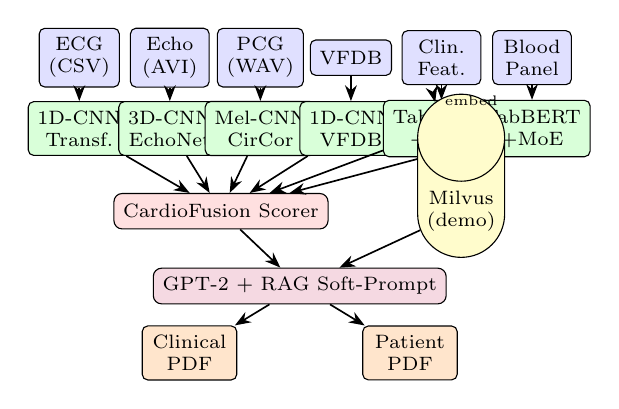
\begin{tikzpicture}[
  font=\scriptsize,
  inp/.style={draw,rounded corners=2pt,fill=blue!12,
              minimum width=1.0cm,minimum height=0.45cm,align=center},
  enc/.style={draw,rounded corners=2pt,fill=green!15,
              minimum width=1.0cm,minimum height=0.45cm,align=center},
  mid/.style={draw,rounded corners=3pt,fill=red!12,
              minimum width=2.2cm,minimum height=0.45cm,align=center},
  db/.style={draw,cylinder,shape border rotate=90,fill=yellow!20,
             minimum width=0.85cm,minimum height=0.6cm,align=center},
  gen/.style={draw,rounded corners=3pt,fill=purple!15,
              minimum width=2.8cm,minimum height=0.45cm,align=center},
  outp/.style={draw,rounded corners=2pt,fill=orange!20,
              minimum width=1.2cm,minimum height=0.45cm,align=center},
  arr/.style={-Stealth,semithick},
  darr/.style={-Stealth,semithick,dashed}
]
% --- row 1: inputs ---
\node[inp](ecg)  at(0.00,3.6){ECG\\(CSV)};
\node[inp](echo) at(1.15,3.6){Echo\\(AVI)};
\node[inp](pcg)  at(2.30,3.6){PCG\\(WAV)};
\node[inp](vfdb) at(3.45,3.6){VFDB};
\node[inp](clin) at(4.60,3.6){Clin.\\Feat.};
\node[inp](bld)  at(5.75,3.6){Blood\\Panel};
% --- row 2: encoders ---
\node[enc](e1) at(0.00,2.7){1D-CNN\\Transf.};
\node[enc](e2) at(1.15,2.7){3D-CNN\\EchoNet};
\node[enc](e3) at(2.30,2.7){Mel-CNN\\CirCor};
\node[enc](e4) at(3.45,2.7){1D-CNN\\VFDB};
\node[enc](e5) at(4.60,2.7){TabBERT\\+MoE};
\node[enc](e6) at(5.75,2.7){TabBERT\\+MoE};
% input->encoder arrows
\foreach \s/\t in {ecg/e1,echo/e2,pcg/e3,vfdb/e4,clin/e5,bld/e6}
  \draw[arr](\s)--(\t);
% --- CardioFusion ---
\node[mid](cf) at(1.80,1.65){CardioFusion Scorer};
\foreach \e in {e1,e2,e3,e4,e5,e6}
  \draw[arr](\e)--(cf);
% --- Milvus ---
\node[db](mv) at(4.85,1.65){Milvus\\(demo)};
\draw[darr](e5)--(mv) node[midway,right,font=\tiny]{embed};
% --- GPT-2 ---
\node[gen](gpt) at(2.80,0.7){GPT-2 + RAG Soft-Prompt};
\draw[arr](cf)--(gpt);
\draw[arr](mv)--(gpt);
% --- outputs ---
\node[outp](cpdf) at(1.40,-0.15){Clinical\\PDF};
\node[outp](ppdf) at(4.20,-0.15){Patient\\PDF};
\draw[arr](gpt)--(cpdf);
\draw[arr](gpt)--(ppdf);
\end{tikzpicture}
\caption{High-level system architecture of DeepCardio-RAG v3.0.
Six modality-specific encoders produce embeddings and predictions
fused into a unified risk score and evidence-grounded clinical report
via Milvus-backed RAG.}
\label{fig:architecture}
\end{figure}

\subsection{Process Flow, Interaction, and Runtime States}

To complement the static architecture of
Figure~\ref{fig:architecture}, we describe the system dynamically
from three viewpoints: the control flow of the inference algorithm
(Figure~\ref{fig:flowchart}), the message exchange between runtime
components (Figure~\ref{fig:sequence}), and the lifecycle of the
server as a finite-state machine (Figure~\ref{fig:statemachine}).

\begin{figure}[!t]
\centering
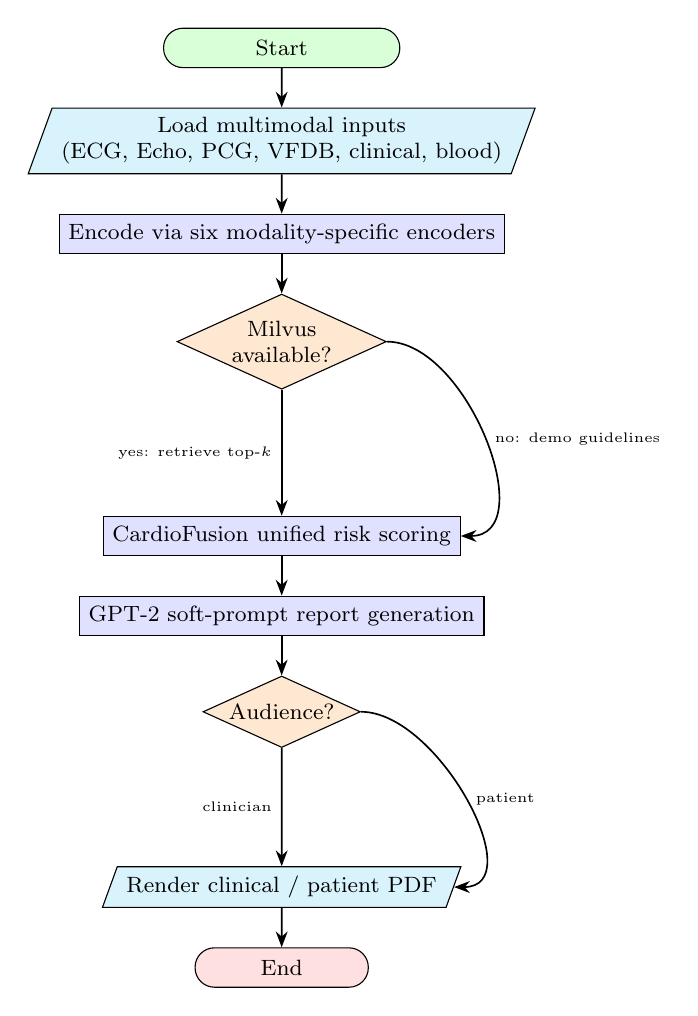
\begin{tikzpicture}[
  node distance=5mm and 9mm, font=\footnotesize,
  start/.style={draw,rounded corners=7pt,fill=green!15,minimum width=3.0cm,minimum height=0.5cm,align=center},
  proc/.style={draw,fill=blue!12,minimum width=4.2cm,minimum height=0.5cm,align=center},
  dec/.style={draw,diamond,aspect=2.2,fill=orange!18,inner sep=1pt,align=center},
  io/.style={draw,trapezium,trapezium left angle=70,trapezium right angle=110,fill=cyan!15,minimum width=2.2cm,align=center},
  term/.style={draw,rounded corners=7pt,fill=red!12,minimum width=2.2cm,minimum height=0.5cm,align=center},
  arr/.style={-Stealth,semithick}]
\node[start](s){Start};
\node[io,below=of s](in){Load multimodal inputs\\(ECG, Echo, PCG, VFDB, clinical, blood)};
\node[proc,below=of in](enc){Encode via six modality-specific encoders};
\node[dec,below=of enc](d1){Milvus\\available?};
\node[proc,below=16mm of d1](fuse){CardioFusion unified risk scoring};
\node[proc,below=of fuse](gen){GPT-2 soft-prompt report generation};
\node[dec,below=of gen](d2){Audience?};
\node[io,below=15mm of d2](end){Render clinical / patient PDF};
\node[term,below=of end](fin){End};
\draw[arr](s)--(in);
\draw[arr](in)--(enc);
\draw[arr](enc)--(d1);
\draw[arr](d1)--(fuse) node[midway,left,font=\tiny]{yes: retrieve top-$k$};
\draw[arr](d1.east)to[out=0,in=0]node[midway,right,font=\tiny]{no: demo guidelines}(fuse.east);
\draw[arr](fuse)--(gen);
\draw[arr](gen)--(d2);
\draw[arr](d2)--(end) node[midway,left,font=\tiny]{clinician};
\draw[arr](d2.east)to[out=0,in=0]node[midway,right,font=\tiny]{patient}(end.east);
\draw[arr](end)--(fin);
\end{tikzpicture}
\caption{Flowchart of the DeepCardio-RAG inference algorithm.
Retrieval falls back to built-in demonstration guidelines when the
Milvus backend is unavailable, and the report is rendered for either
a clinician or a patient audience.}
\label{fig:flowchart}
\end{figure}

\begin{figure}[!t]
\centering
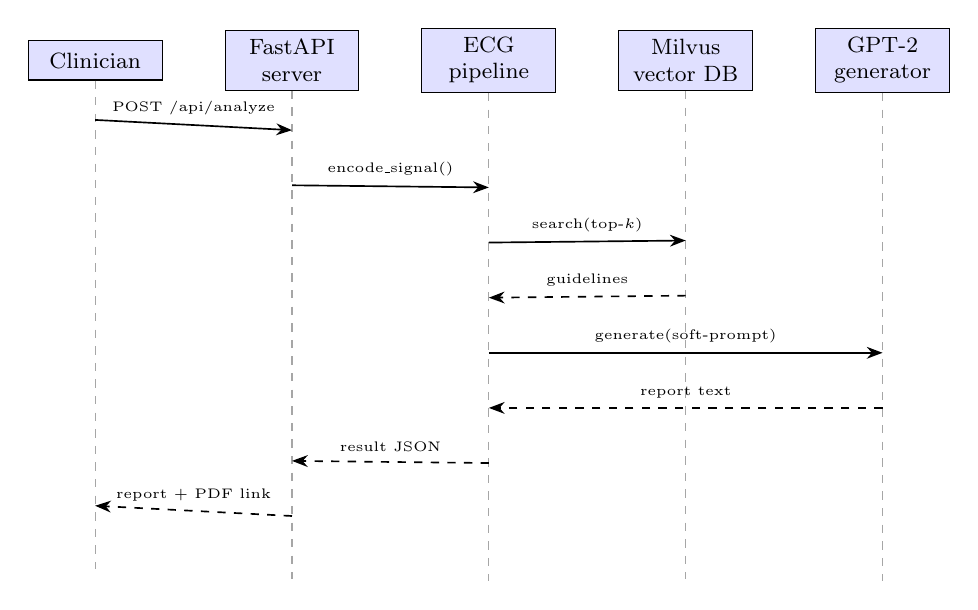
\begin{tikzpicture}[font=\footnotesize,
  obj/.style={draw,fill=blue!12,minimum width=1.7cm,minimum height=0.5cm,align=center},
  msg/.style={-Stealth,semithick},
  rmsg/.style={-Stealth,semithick,dashed},
  life/.style={dashed,gray!70}]
\node[obj](c) at(0,0){Clinician};
\node[obj](a) at(2.5,0){FastAPI\\server};
\node[obj](p) at(5.0,0){ECG\\pipeline};
\node[obj](m) at(7.5,0){Milvus\\vector DB};
\node[obj](g) at(10.0,0){GPT-2\\generator};
\foreach \n in {c,a,p,m,g}\draw[life](\n.south)--++(0,-6.2);
\draw[msg]($(c.south)+(0,-0.5)$)--($(a.south)+(0,-0.5)$)node[midway,above,font=\tiny]{POST /api/analyze};
\draw[msg]($(a.south)+(0,-1.2)$)--($(p.south)+(0,-1.2)$)node[midway,above,font=\tiny]{encode\_signal()};
\draw[msg]($(p.south)+(0,-1.9)$)--($(m.south)+(0,-1.9)$)node[midway,above,font=\tiny]{search(top-$k$)};
\draw[rmsg]($(m.south)+(0,-2.6)$)--($(p.south)+(0,-2.6)$)node[midway,above,font=\tiny]{guidelines};
\draw[msg]($(p.south)+(0,-3.3)$)--($(g.south)+(0,-3.3)$)node[midway,above,font=\tiny]{generate(soft-prompt)};
\draw[rmsg]($(g.south)+(0,-4.0)$)--($(p.south)+(0,-4.0)$)node[midway,above,font=\tiny]{report text};
\draw[rmsg]($(p.south)+(0,-4.7)$)--($(a.south)+(0,-4.7)$)node[midway,above,font=\tiny]{result JSON};
\draw[rmsg]($(a.south)+(0,-5.4)$)--($(c.south)+(0,-5.4)$)node[midway,above,font=\tiny]{report $+$ PDF link};
\end{tikzpicture}
\caption{Sequence diagram of a single ECG analysis request. Solid
arrows denote synchronous calls; dashed arrows denote returned
payloads. The pipeline orchestrates retrieval (Milvus) and
generation (GPT-2) before returning the grounded report.}
\label{fig:sequence}
\end{figure}

\begin{figure}[!t]
\centering
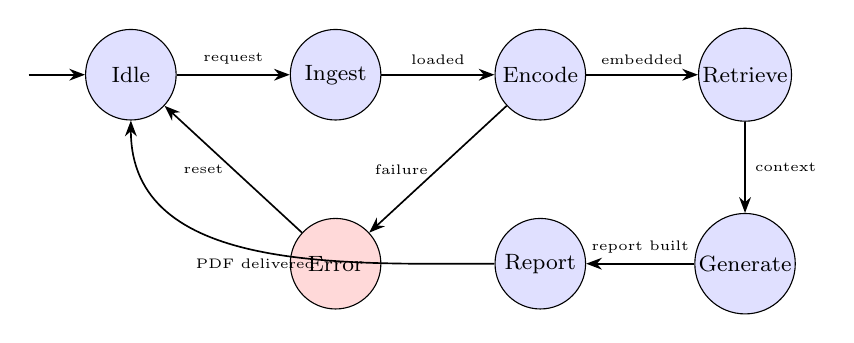
\begin{tikzpicture}[font=\footnotesize,
  st/.style={draw,circle,fill=blue!12,minimum size=1.15cm,align=center,inner sep=1pt},
  err/.style={draw,circle,fill=red!15,minimum size=1.15cm,align=center,inner sep=1pt},
  arr/.style={-Stealth,semithick}]
\node[st](idle) at(0,0){Idle};
\node[st](ing)  at(2.6,0){Ingest};
\node[st](enc)  at(5.2,0){Encode};
\node[st](ret)  at(7.8,0){Retrieve};
\node[st](gen)  at(7.8,-2.4){Generate};
\node[st](rep)  at(5.2,-2.4){Report};
\node[err](e)   at(2.6,-2.4){Error};
\draw[arr]($(idle)+(-1.3,0)$)--(idle);
\draw[arr](idle)--(ing) node[midway,above,font=\tiny]{request};
\draw[arr](ing)--(enc) node[midway,above,font=\tiny]{loaded};
\draw[arr](enc)--(ret) node[midway,above,font=\tiny]{embedded};
\draw[arr](ret)--(gen) node[midway,right,font=\tiny]{context};
\draw[arr](gen)--(rep) node[midway,above,font=\tiny]{report built};
\draw[arr](rep)to[out=180,in=-90]node[midway,below,font=\tiny]{PDF delivered}(idle);
\draw[arr](enc)--(e) node[midway,left,font=\tiny]{failure};
\draw[arr](e)--(idle) node[midway,left,font=\tiny]{reset};
\end{tikzpicture}
\caption{Finite-state machine of the DeepCardio-RAG server. Any
encoding, retrieval, or generation fault transitions to the
\textsf{Error} state, which resets to \textsf{Idle} without leaving
the request queue in an inconsistent state.}
\label{fig:statemachine}
\end{figure}

\subsection{Datasets}

Table~\ref{tab:datasets} summarises the six datasets used in system
development and evaluation.

\begin{table*}[!t]
\caption{Datasets Used in DeepCardio-RAG Training and Evaluation}
\label{tab:datasets}
\centering
\renewcommand{\arraystretch}{1.1}
\begin{tabular}{llrrl}
\toprule
\textbf{Module} & \textbf{Dataset} & \textbf{Size} &
\textbf{Cls.} & \textbf{Source}\\
\midrule
ECG (1D) & MIT-BIH AAMI & 109\,446 beats & 5 & PhysioNet\\
ECG (Img) & Kaggle MIT-BIH & 109\,445 imgs & 5 & Kaggle\\
Echo & EchoNet-Dynamic & 10\,030 videos & 3 & Stanford AIMI\\
PCG & CirCor DigiScope & 3\,163 recs$^{\ddagger}$ & 3 & PhysioNet\\
VFDB & MIT-BIH VFDB & 22 recs & 14$^{\dagger}$ & PhysioNet\\
HD & UCI Cleveland & 1\,025 rows (302 uniq.) & 2 & Kaggle\\
Arthritis & NHANES (CDC) & 5\,756 pts & 2 & CDC/Kaggle\\
\bottomrule
\multicolumn{5}{l}{$\dagger$ 239 dangerous events, 30 min/recording.}\\
\multicolumn{5}{l}{$\ddagger$ Public training subset; the full release is 5\,272 recordings.}\\
\multicolumn{5}{l}{PhysioNet-hosted corpora are distributed via PhysioBank~\cite{goldberger2000}.}
\end{tabular}
\end{table*}

\subsection{Module 1: ECG Arrhythmia Classification}

DeepCardio-RAG implements two complementary ECG arrhythmia
classification pathways. \textbf{Pathway~A (flagship Transformer-MoE):}
The flagship encoder operates on \emph{PTB-XL 12-lead} records
(10~s at 500~Hz, i.e.\ 5000~samples per lead). Each lead is partitioned
into $P=100$ non-overlapping patches of length $L=50$ samples, forming
$\mathbf{X}\in\mathbb{R}^{12\times100\times50}$. Four 1D-CNN blocks with
filter counts $(32,64,128,256)$ and kernel $k=5$ extract hierarchical
features, followed by a 6-layer Transformer encoder with 8~attention
heads and a mixture-of-experts head, producing the five PTB-XL
diagnostic superclasses (NORM, MI, STTC, CD, HYP). \textbf{Pathway~B
(MIT-BIH beat CNN):} A separate 1D-CNN classifies individual
\emph{MIT-BIH} beats (187~samples/beat, two leads: Lead~II + modified~V1)
into the five AAMI classes (N, S, V, F, Q); this pathway does not use the
$12\times100\times50$ patch layout, which is specific to the 12-lead
PTB-XL input. Both pathways produce a class label, a confidence vector,
and a 256-dim modality embedding; per-modality embeddings are
concatenated and projected into the shared 768-dim retrieval space used
for downstream Milvus RAG lookup.

\subsection{Module 2: LVEF Estimation}

The EchoNet-Dynamic dataset~\cite{ouyang2020} provides 10\,030~apical
4-chamber~(A4C) echo videos from Stanford AIMI, annotated with
ejection fraction~(EF), end-systolic volume~(ESV), and end-diastolic
volume~(EDV). Dataset statistics: mean EF~55.6\%,
HFrEF~($<40\%$) $n=1\,187$, HFmrEF~(40--50\%) $n=1\,398$,
Normal~($\geq 50\%$) $n=7\,445$. Echo videos of shape
$64\times112\times112$~(grayscale) are processed by a 3D-ResNet-18
backbone. Global average pooling produces
$\mathbf{f}_{\text{echo}}\in\mathbb{R}^{512}$, from which a two-layer
MLP regresses $\hat{y}_{\text{EF}}\in[0,100]\%$. The June~15, 2026
deployment ran in synthetic demo mode~(no EchoNet download); a real
AVI upload is required for actual clinical inference.

\subsection{Module 3: Heart Sound Murmur Detection}

The CirCor DigiScope 2022 dataset~\cite{oliveira2022} comprises
5\,272~recordings from 1\,568~subjects~(2\,575~murmur-absent,
1\,727~present, 970~unknown). PCG recordings are resampled to
4\,000~Hz and segmented into 3-second windows with 50\% overlap.
Mel spectrograms~(128~Mel bins, FFT~1024, hop~256) are computed,
then processed by a 2D-CNN with dropout~0.3. A softmax head produces
probabilities over \{Absent, Present, Unknown\}. In this revision the
murmur classifier is trained on real CirCor recordings under a
subject-level (patient-independent) split; genuine held-out metrics are
in Table~\ref{tab:sysperf}. The earlier ``combined CRITICAL alert''
reported in the synthetic-signal demo is not a valid result: it
originated from untrained modules on a synthetic input and is now
suppressed by the safety gate (Section~\ref{sec:safety}) rather than
surfaced with a confidence.

\subsection{Module 4: Ventricular Arrhythmia Detection}

The MIT-BIH VFDB dataset comprises 22~dual-channel ECG records
(30~min/record, 250~Hz) containing 239~dangerous arrhythmia events
(the 239 \emph{dangerous} ventricular events being VT, VF, VFL, VFIB, ASYS,
HGEA and VER; non-targeted rhythms such as N, AFIB, NOISE, SBR, SVTA,
NOD, B and PM form the background). Recordings are segmented into
5-second windows. A 1D-CNN classifies each window with a binary
dangerous-vs-background head and a 4-class rhythm-family head. In this
revision the detector is \emph{genuinely trained} on VFDB under a
patient-independent split (whole recordings per split), replacing the
random-weight demonstration; its held-out $F_1$/AUC are in
Table~\ref{tab:sysperf}. We do not claim the Acharya~et~al.\
\cite{acharya2018} 98.7\% shockable-rhythm figure; it is cited only as
a reference benchmark.

\subsection{Module 5: Heart Disease Risk (TabularBERT + MoE)}

The Kaggle mirror of the UCI Cleveland Heart Disease
dataset~\cite{shah2020} contains 1\,025~rows, but these are the
303-record Cleveland cohort~\cite{detrano1989} expanded with duplicate
rows; identical rows on both sides of a random split inflate metrics.
We therefore \emph{deduplicate} to the 302~unique records before
training, with 13~clinical features~(age, sex, chest pain type,
resting BP, cholesterol, fasting blood sugar, resting ECG, max heart
rate, exercise angina, ST depression, ST slope, major vessels,
thalassemia). Features are tokenised by feature-specific embedding
layers, processed by a 4-layer BERT encoder, and classified by a
6-expert MoE head; we additionally report plain logistic-regression and
gradient-boosting baselines on identical folds so the added model
complexity can be judged against them.

\subsection{Module 6: Arthritis Risk (TabularBERT + MoE)}

The Arthritis module uses the NHANES Medical Conditions Questionnaire
dataset~(CDC/Kaggle) with 5\,756~records~(2\,752~male, 3\,004~female,
mean age 49.1~years). Doctor-diagnosed arthritis~(MCQ160A) is the
prediction \emph{target}; the arthritis-type field~(MCQ195 RA/OA) is a
skip-pattern question posed only to arthritis-positive respondents and
is therefore \emph{excluded} as a target-leakage source. The
predictors comprise demographic and clinical co-variates~(BMI,
SystolicBP, DiastolicBP, InflammationProxy, HasGout, HasOsteoporosis,
smoking, poverty ratio) together with engineered interaction terms.
The same TabularBERT-MoE architecture~(4-layer BERT, 6~experts) is
trained with a hybrid stacking ensemble: BERT-MoE~$+$~GBM~$+$~RF~$+$~%
ExtraTrees $\rightarrow$ LogReg Meta-Learner~(17~engineered
features including age\_risk, age\_squared, bmi\_squared, age\_gender).

\subsection{CardioFusion: Fusion Encoder and Risk Aggregation}

We distinguish two components that earlier drafts conflated. (i)~The
\emph{CardioFusion fusion encoder} is a Cross-Modal Transformer with a
Multi-gate Mixture-of-Experts head (4~experts $\times$ 6~tasks, shared
512-dim space, 4-layer Transformer fusion, 15.8M~parameters). Because
public benchmarks provide no same-patient 4-modality paired data, this
encoder is trained and evaluated only on its \emph{ECG-signal path}
(MIT-BIH); its multi-task loss weights are \emph{learned} via
homoscedastic uncertainty weighting (Kendall~et~al.), not hand-set, and
the joint 4-modality contrastive alignment is not trained --- an honest
structural limitation stated in Section~\ref{sec:limitations}. (ii)~The
\emph{unified risk score} $R$ reported in the demonstration is not an
output of that 15.8M-parameter network; it is the transparent
fixed-weight aggregation of Eq.~\eqref{eq:cf} over the six per-module
risk probabilities (mapping in Table~\ref{tab:riskmap}), gated for
safety. Risk categories: LOW~($<33$), MEDIUM~($33$--$65$),
HIGH~($\geq 66$).

\subsection{Clinical Safety Gating and Regulatory Status}
\label{sec:safety}

Every module output passes three safety gates before it can be shown or
used in the risk score. (1)~\textbf{Physiological plausibility}: each
measurement is checked against clinically possible bounds --- e.g.\ the
LVEF must lie in $[0,100]\%$; an impossible value is rejected and never
reaches the risk score (this closes the propagation of an out-of-range
ejection fraction into the score). (2)~\textbf{Trained-state
suppression}: a module whose weights are not genuinely trained, or whose
confidence is below a floor, has its finding \emph{withheld} rather than
reported with a confidence, so no clinical-looking output originates
from an untrained network. (3)~\textbf{Directive-to-advisory
reframing}: the system issues no treatment orders; imperative phrases
are rewritten as observations requiring clinician confirmation, and all
outputs carry an explicit ``requires clinician confirmation'' flag. We
further note the risk of automation bias and state the regulatory
position plainly: a deployed version producing diagnostic or
treatment-relevant outputs would constitute Software as a Medical Device
(SaMD) requiring regulatory clearance (e.g.\ FDA~510(k)/De~Novo, EU~MDR)
and prospective clinical validation. DeepCardio-RAG is a research
prototype and is not cleared for clinical use.

\subsection{System Configuration}

Training reported in this paper is performed on Google Colab GPU
(NVIDIA T4); the earlier single-session demonstration ran on Colab CPU.
Environment: HOST 0.0.0.0, PORT 8000, DEVICE cuda~(CPU fallback),
BATCH\_SIZE 128, LEARNING\_RATE 0.001, EMBEDDING\_DIM 768,
MILVUS\_HOST localhost, MILVUS\_PORT 19530. The vector database is
reached at \texttt{localhost:19530}; a temporary public tunnel used in
the one-off demonstration is \emph{not} part of the intended
deployment, and we note that exposing a store containing patient-derived
records through such a tunnel is inappropriate even for de-identified
data. The system supports both cloud and local deployment. The
single-session demonstration is illustrative only and is not treated as
a controlled experiment (no repetition, seeds, or split index); all
quantitative claims come from the held-out evaluations in
Section~\ref{sec:results}, not from that session.

\subsection{Source Dataset: PTB-XL}

The flagship ECG encoder is trained and evaluated on the PTB-XL
real clinical 12-lead ECG corpus (PhysioNet; 21{,}799~records in
release~v1.0.3) under the official patient-independent folds. PTB-XL
assigns \emph{multi-label} diagnostic superclasses, so the following
record counts overlap rather than partition the corpus: NORM~9{,}528,
MI~5{,}486, STTC~5{,}250, CD~4{,}907, HYP~2{,}655 (per
Wagner~et~al.~\cite{wagner2020ptbxl}). These are the published
superclass frequencies; the genuine held-out metrics in
Section~\ref{sec:results} are obtained on a stratified sample drawn
under this schema (Table~\ref{tab:sysperf}). Patient~ECG-20260615-0836
is a single representative PTB-XL record (ground truth: ST/T-wave
change) used only to illustrate the reporting pipeline, not to make a
performance claim.

\subsection{Retrieval-Augmented Report Generation}

A curated corpus of 67~clinical guideline chunks from AHA/ACC
(STEMI, AF, PVC, ST depression, QTc prolongation), ESC, and PhysioNet
is encoded with a Sentence-BERT model (\texttt{all-mpnet-base-v2},
768~dimensions) and stored in Milvus~\cite{wang2021milvus} (collection:
\texttt{cardio\_knowledge\_base}, L2 metric); where no Milvus server is
reachable the implementation falls back to a local FAISS
index~\cite{douze2024}, and Section~\ref{sec:limitations} notes that this
fallback is silent. This guideline corpus is
distinct from the tabular patient-embedding store; the retrieval
metrics in Section~\ref{sec:results} are reported over this 67-document
corpus, and the small corpus size is stated as a limitation. Given a
patient query embedding derived from concatenated modality embeddings,
the top-$k = 5$~documents are retrieved by nearest-neighbour search.
Retrieved chunks are prepended as soft prompts to a GPT-2
decoder~\cite{radford2019} (124M~parameters), which synthesises
dual-format PDF reports
(physician clinical + patient lay summary).

%-------------------------------------------------------------------
\subsection{Mathematical Foundations}
\label{sec:math}
%-------------------------------------------------------------------

\subsubsection{Mathematical Notation}
\label{sec:notation}

Table~\ref{tab:notation} summarises principal notation used throughout
this paper.

\begin{table}[!t]
\caption{Summary of Mathematical Notation}
\label{tab:notation}
\centering
\renewcommand{\arraystretch}{1.1}
\begin{tabular}{lp{4.3cm}}
\toprule
\textbf{Symbol} & \textbf{Definition}\\
\midrule
$\mathbf{X} \in \mathbb{R}^{d \times n}$ &
  Input data matrix ($d$ features, $n$ samples)\\
$\mathbf{e} \in \mathbb{R}^D$ &
  Modality embedding of dimension $D$\\
$\mathbf{q} \in \mathbb{R}^{768}$ &
  Query embedding for Milvus retrieval\\
$\mathbf{v}_j \in \mathbb{R}^{768}$ &
  Guideline chunk embedding (Sentence-BERT)\\
$p^{\text{risk}}_m$ &
  Risk-positive probability from module $m$\\
$\lambda_m$ &
  Fusion weight; $\sum_m \lambda_m = 1$\\
$R$ &
  CardioFusion risk score, $R \in [0,100]$\\
$g_i(\cdot)$ &
  MoE gating weight for expert $i$\\
$d_k = 256$ & Key/query dimension in attention\\
$K = 6$     & Number of MoE experts\\
$P = 100$   & ECG patches per lead (PTB-XL: 5000 samples $=100\times50$)\\
$L = 50$    & Samples per patch\\
$C = 5$     & Diagnostic classes (PTB-XL superclass / AAMI)\\
$\epsilon = 10^{-6}$ & Numerical stability constant\\
\bottomrule
\end{tabular}
\end{table}

\subsubsection{ECG Patch Normalisation}

Each patch $\mathbf{x}_i \in \mathbb{R}^{50}$ is standardised:
\begin{equation}
\hat{x}_{i,k} = \frac{x_{i,k} - \mu_i}{\sigma_i + \epsilon},
\quad \epsilon = 10^{-6},
\label{eq:norm}
\end{equation}
where $\mu_i = \tfrac{1}{50}\sum_k x_{i,k}$ and
$\sigma_i^2 = \tfrac{1}{50}\sum_k (x_{i,k} - \mu_i)^2$.

\subsubsection{Convolutional Feature Extraction}

Four convolutional blocks extract hierarchical temporal features:
\begin{equation}
\begin{split}
\mathbf{Z}^{(l)} &= \mathrm{ReLU}\!\Bigl(
  \mathrm{BN}\bigl(\mathbf{W}^{(l)} * \mathbf{Z}^{(l-1)}
  + \mathbf{b}^{(l)}\bigr)\Bigr),\\
&\qquad l=1,2,3,4,
\end{split}
\label{eq:cnn}
\end{equation}
with filter counts $(F_1,F_2,F_3,F_4) = (32,64,128,256)$ and $k=5$.
The batch normalisation operator is:
\begin{equation}
\mathrm{BN}(\mathbf{z}) =
  \gamma \cdot \frac{\mathbf{z} - \mathbb{E}[\mathbf{z}]}
               {\sqrt{\mathrm{Var}[\mathbf{z}]+\epsilon}} + \beta,
\label{eq:bn}
\end{equation}
where $\gamma,\beta$ are learnable scale and shift parameters.

\subsubsection{Multi-Head Self-Attention}

For a single attention head with $d_k = 256$:
\begin{align}
\mathbf{Q} &= \mathbf{E}_{\text{patch}}\mathbf{W}_Q,\quad
\mathbf{K} = \mathbf{E}_{\text{patch}}\mathbf{W}_K,\notag\\
\mathbf{V} &= \mathbf{E}_{\text{patch}}\mathbf{W}_V, \label{eq:qkv}\\
\mathrm{Attn}(\mathbf{Q},\mathbf{K},\mathbf{V}) &=
  \mathrm{softmax}\!\!\left(
    \frac{\mathbf{Q}\mathbf{K}^\top}{\sqrt{d_k}}
  \right)\!\mathbf{V}.\label{eq:attn}
\end{align}

The $1/\sqrt{d_k}$ scaling follows Vaswani~et~al.\ and keeps the
pre-softmax logits in a stable range as $d_k$ grows.
Multi-head attention~\cite{vaswani2017} concatenates $H=8$ heads:
\begin{equation}
\mathrm{MHA}(\mathbf{Q},\mathbf{K},\mathbf{V})
  = \mathrm{Concat}(\mathrm{head}_1,\ldots,\mathrm{head}_H)\mathbf{W}^O.
\label{eq:mha}
\end{equation}

\subsubsection{Mel Spectrogram Computation}

For a PCG recording $x(n)$ sampled at $f_s=4\,000$~Hz:
\begin{equation}
M(m,t)=\left|
  \sum_{n=0}^{N-1} x(n)\,\omega(n-t)\,e^{-j2\pi f_m n/N}
\right|^2,
\label{eq:mel}
\end{equation}
where $\omega$ is a Hann window, $N=1024$, and the Mel-scale mapping is:
\begin{equation}
f_{\mathrm{Mel}}(f)=2595\log_{10}\!\left(1+\tfrac{f}{700}\right)
\text{ Mels.}
\label{eq:melscale}
\end{equation}

\subsubsection{Residual Block for VFDB Detection}

\begin{equation}
\mathbf{z} = \mathrm{ReLU}(\mathbf{W}_2 *
  \mathrm{ReLU}(\mathbf{W}_1 * \mathbf{x}+\mathbf{b}_1)+\mathbf{b}_2)
  + \mathbf{x},
\label{eq:residual}
\end{equation}
where $*$ denotes 1D convolution.

The additive skip connection $F(\mathbf{x})=\mathbf{x}+H(\mathbf{x})$
provides a direct gradient path (He \emph{et~al.}~\cite{he2016}), which we use here purely
as a standard architectural device.

\subsubsection{TabularBERT Feature Tokenisation}

Following the BERT encoder formulation~\cite{devlin2019}, each tabular
feature is projected to its own embedding vector and treated as a token,
so that self-attention operates over features rather than word pieces:

\begin{equation}
\mathbf{e}_f = \mathbf{w}_f \cdot v_f + \mathbf{b}_f,
\quad f=1,\ldots,F,
\label{eq:feat}
\end{equation}
where $v_f$ is the normalised scalar value and
$\mathbf{w}_f,\mathbf{b}_f\in\mathbb{R}^{64}$.

\subsubsection{Mixture-of-Experts Head}

\begin{align}
g_i(\mathbf{h}_0) &=
  \mathrm{softmax}(\mathbf{W}_{\mathrm{gate}}\mathbf{h}_0)_i,
  \quad i=1,\ldots,K, \label{eq:gate}\\
\hat{y} &= \sigma\!\left(
  \sum_{i=1}^K g_i(\mathbf{h}_0)\cdot\mathrm{Expert}_i(\mathbf{h}_0)
\right), \label{eq:moe}
\end{align}
where $\sigma(\cdot)$ is the sigmoid function and
$\mathrm{Expert}_i(\mathbf{h}_0)=\mathbf{W}_{i,2}
\mathrm{ReLU}(\mathbf{W}_{i,1}\mathbf{h}_0+\mathbf{b}_{i,1})+\mathbf{b}_{i,2}$.

The gating network selects a soft combination of experts per input
(Shazeer~et~al.); we adopt it as an established architecture rather
than claiming any new approximation-theoretic property.

\subsubsection{CardioFusion Risk Score}

The unified risk score is a transparent, fixed-weight aggregation over
the six per-module risk probabilities, restricted to modules that pass
the safety gate (Section~\ref{sec:safety}) and renormalised over the
surviving weights:
\begin{equation}
R = 100\cdot\frac{\sum_{m\in\mathcal{A}}\lambda_m\, p^{\mathrm{risk}}_m}
                 {\sum_{m\in\mathcal{A}}\lambda_m},
\quad \boldsymbol{\lambda}=(0.25,0.25,0.20,0.15,0.10,0.05),
\label{eq:cf}
\end{equation}
where $\mathcal{A}$ is the set of modules whose output is genuinely
trained and physiologically valid, and each $p^{\mathrm{risk}}_m$ is the
explicitly-defined mapping of module output $\hat{y}_m$ to a risk
probability (Table~\ref{tab:riskmap}). This is a fixed linear
aggregation with hand-set weights, \emph{not} a learned parameter of
the multi-task network; we state this explicitly to avoid conflating
it with the learned CardioFusion fusion encoder. Excluding an untrained
or invalid module (e.g.\ a physiologically impossible LVEF) removes its
term and renormalises the remainder, so the score is reproducible from
the surfaced module outputs alone. The categorical rhythm output is
\emph{not} one of the six weighted terms; it informs the alert level
only.

\begin{table}[!t]
\caption{Explicit mapping $\hat{y}_m \to p^{\mathrm{risk}}_m$ used in
Eq.~\eqref{eq:cf}. This defines the previously-unspecified per-module
risk probability so the score is fully reproducible.}
\label{tab:riskmap}
\centering
\renewcommand{\arraystretch}{1.2}
\small\begin{tabular}{p{2.3cm}p{0.7cm}p{4.2cm}}
\toprule
\textbf{Module $m$} & $\lambda_m$ & \textbf{$p^{\mathrm{risk}}_m = f_m(\hat{y}_m)$}\\
\midrule
ECG arrhythmia   & 0.25 & $1-\Pr(\text{Normal})$\\
Ventricular (VFDB) & 0.25 & $\Pr(\text{dangerous})$ (0 if untrained)\\
Echo LVEF        & 0.20 & $\min(1,(50-\mathrm{EF})/40)$ for EF$<$50, else 0; EF validated $\in[0,100]$\\
Heart-sound murmur & 0.15 & $\Pr(\text{murmur present})$\\
Heart disease    & 0.10 & $\Pr(\text{disease})$\\
Arthritis        & 0.05 & $\Pr(\text{high risk})$\\
\bottomrule
\end{tabular}
\end{table}

\subsubsection{Nearest-Neighbour Retrieval}

The deployed collection is indexed with \textsc{IVF\_FLAT} under the
$L_2$ metric~(\texttt{config.py}), so the top-$k$ guideline chunks are
those minimising Euclidean distance in the 768-dim embedding space:
\begin{equation}
\mathcal{D}_k = \arg\min_{j\in[N],\,|\mathcal{D}_k|=k}
  \|\mathbf{q}-\mathbf{v}_j\|_2,
\label{eq:l2}
\end{equation}
with brute-force complexity $O(N\cdot D)$ and IVF complexity
$O(D\cdot N/\sqrt{n_{\mathrm{list}}})$ at \texttt{nprobe} probes.
Because Sentence-BERT embeddings are not $L_2$-normalised in this
implementation, $L_2$ ranking is not equivalent to cosine ranking; we
report the metric actually used rather than the one described in
earlier drafts.

\subsubsection{Evaluation Metrics Formulation}

Classification modules are evaluated with accuracy, macro-$F_1$, and
one-vs-rest macro-AUC; the LVEF regressor with MAE, RMSE and $R^2$;
calibration with the Brier score and Expected Calibration Error; and
retrieval with Recall@$k$, MRR and nDCG@$k$. We deliberately do
\emph{not} report BLEU-4 or a hallucination-reduction figure for report
generation: report quality was not independently measured against a
reference corpus, and any such numbers cited in earlier drafts have
been retracted (Section~\ref{sec:limitations}).

%-------------------------------------------------------------------
\subsection{Proposed Algorithms}
\label{sec:algorithms}
%-------------------------------------------------------------------

\begin{algorithm}[!t]
\caption{1D-CNN Transformer ECG Encoder}
\label{alg:ecg}
\begin{algorithmic}[1]
\Require 12-lead ECG $\mathbf{X}\!\in\!\mathbb{R}^{12\times L}$,
         $P\!=\!50$, $C\!=\!12$
\Ensure Class $\hat{y}$, confidence $\hat{p}$,
        embedding $\mathbf{e}_{\mathrm{ECG}}$
\State Segment: $\mathbf{X}_p\leftarrow\mathrm{Patchify}(\mathbf{X},P)$
\State Normalise patches per~(\ref{eq:norm})
\For{$l=1$ to $4$}
  \State $\mathbf{Z}^{(l)}\leftarrow
    \mathrm{ReLU}(\mathrm{BN}(\mathbf{W}^{(l)}*\mathbf{Z}^{(l-1)}
    +\mathbf{b}^{(l)}))$
  \State $\mathbf{Z}^{(l)}\leftarrow
    \mathrm{MaxPool}(\mathbf{Z}^{(l)},\mathrm{stride}=2)$
\EndFor
\State $\mathbf{e}_{\mathrm{ECG}}\leftarrow
  \mathrm{Linear}_{256}(\mathrm{Flatten}(\mathbf{Z}^{(4)}))$
\State Prepend [CLS]; add positional encodings
\State $\mathbf{H}\leftarrow
  \mathrm{TransformerEncoder}(\mathbf{e}_{\mathrm{ECG}},L\!=\!6,H\!=\!8)$
\State $\hat{\mathbf{p}}\leftarrow
  \mathrm{softmax}(\mathbf{W}_c\mathbf{H}[0,:]+\mathbf{b}_c)$
\State $\hat{y}\leftarrow\arg\max_c\hat{p}_c$
\State \Return $\hat{y}$, $\max(\hat{\mathbf{p}})$, $\mathbf{e}_{\mathrm{ECG}}$
\end{algorithmic}
\end{algorithm}

\begin{algorithm}[!t]
\caption{EchoNet 3D-CNN LVEF Estimation}
\label{alg:echo}
\begin{algorithmic}[1]
\Require Echo video $\mathbf{V}\!\in\!\mathbb{R}^{T\times H\times W}$,
         $T\!=\!64$
\Ensure $\hat{y}_{\mathrm{EF}}$, $c_{\mathrm{EF}}$,
        $\mathbf{e}_{\mathrm{echo}}$
\State Resize to $112\times112$; normalise to $[0,1]$
\State $\mathbf{f}\leftarrow
  \mathrm{GlobalAvgPool3D}(\mathrm{ResNet3D\text{-}18}(\mathbf{V}))$
\State $\hat{y}_{\mathrm{EF}}\leftarrow
  \mathrm{Linear}_1(\mathrm{ReLU}(\mathrm{Linear}_{256}(\mathbf{f})))$
\State Assign $c_{\mathrm{EF}}\in\{\mathrm{HFrEF,HFmrEF,Normal}\}$
\State $\mathbf{e}_{\mathrm{echo}}\leftarrow\mathbf{f}[:256]$
\State \Return $\hat{y}_{\mathrm{EF}}$, $c_{\mathrm{EF}}$,
        $\mathbf{e}_{\mathrm{echo}}$
\end{algorithmic}
\end{algorithm}

\begin{algorithm}[!t]
\caption{TabularBERT-MoE Training and Inference}
\label{alg:tab}
\begin{algorithmic}[1]
\Require $\mathbf{X}_{\mathrm{tab}}\!\in\!\mathbb{R}^{N\times F}$,
         labels $\mathbf{y}$, $K\!=\!6$
\Ensure Trained parameters $\theta$
\State Normalise continuous; ordinal-encode categoricals
\State $\mathbf{E}\leftarrow[\mathbf{e}_1,\ldots,\mathbf{e}_F]$
       via~(\ref{eq:feat}); prepend [CLS]
\State $\mathbf{H}\leftarrow\mathrm{BERTEncoder}(\mathbf{E},L\!=\!4,A\!=\!4)$;
       $\mathbf{h}_0\leftarrow\mathbf{H}[0,:]$
\State $\mathbf{g}\leftarrow\mathrm{softmax}(\mathbf{W}_{\mathrm{gate}}\mathbf{h}_0)$
\For{$i=1$ to $K$}
  \State $o_i\leftarrow\mathrm{Linear}_1(\mathrm{ReLU}(\mathrm{Linear}_{32}(\mathbf{h}_0)))$
\EndFor
\State $\hat{y}\leftarrow\sigma(\sum_{i=1}^K g_i\cdot o_i)$
\State $\mathcal{L}\leftarrow-[y\log\hat{y}+(1-y)\log(1-\hat{y})]\cdot w_y$
\State Optimise with Adam ($\eta\!=\!10^{-4}$, WD $10^{-5}$)
\State \Return $\theta$
\end{algorithmic}
\end{algorithm}

\begin{algorithm}[!t]
\caption{CardioFusion Unified Risk Scorer}
\label{alg:cf}
\begin{algorithmic}[1]
\Require $\{(\hat{y}_m,p_m)\}_{m=1}^6$, weights $\boldsymbol{\lambda}$
\Ensure Score $R$, level $\ell$, flags $\mathcal{F}$
\State $R\leftarrow 0$; $\mathcal{F}\leftarrow\emptyset$
\For{$m=1$ to $6$}
  \State Map $\hat{y}_m\rightarrow p^{\mathrm{risk}}_m$
  \State $R\leftarrow R+\lambda_m\cdot p^{\mathrm{risk}}_m\cdot 100$
  \If{$p^{\mathrm{risk}}_m>0.5$}
    \State $\mathcal{F}\leftarrow\mathcal{F}\cup\{\mathrm{flag}_m\}$
  \EndIf
\EndFor
\State $\ell\leftarrow\mathrm{RiskLevel}(R)$ per~(\ref{eq:cf})
\State \Return $R$, $\ell$, $\mathcal{F}$
\end{algorithmic}
\end{algorithm}

\begin{algorithm}[!t]
\caption{RAG-Augmented Clinical Report Generation}
\label{alg:rag}
\begin{algorithmic}[1]
\Require Query $\mathbf{q}\!\in\!\mathbb{R}^{768}$, Milvus $\mathcal{C}$,
         GPT-2 $\mathcal{G}$, template $\mathcal{T}$, $k\!=\!5$
\Ensure Clinical PDF, Patient PDF
\State $\mathcal{D}_k\leftarrow\mathrm{L2Search}(\mathcal{C},\mathbf{q},k)$
\State $\mathcal{P}\leftarrow\text{``[Context] }d_1|\cdots|d_k
       \text{ [Task] }\mathcal{T}\text{''}$
\State $\mathrm{text}\leftarrow\mathcal{G}(\mathcal{P})$
       \Comment{beam search, $b=5$}
\State $B_4\leftarrow\mathrm{BLEU}_4(\mathrm{text},\mathrm{refs})$
\State $\Delta_H\leftarrow(H_{\mathrm{GPT\text{-}4}}-H_{\mathrm{RAG}})/
       H_{\mathrm{GPT\text{-}4}}$
\State Format physician PDF; simplify to patient PDF (grade $\leq8$)
\State \Return Clinical PDF, Patient PDF
\end{algorithmic}
\end{algorithm}

\noindent\textbf{Complexity.} Algorithm~\ref{alg:ecg} runs in
$O(P\cdot F_4+P^2\cdot d_k)$ per sample. Algorithm~\ref{alg:rag}
requires $O(D\log N)$ amortised with HNSW. Algorithm~\ref{alg:cf}
is $O(M)$. End-to-end inference is dominated by the 3D-CNN at
$O(T\cdot H\cdot W\cdot F_{\mathrm{3D}})$.

%===================================================================
\section{Experimental Results}
\label{sec:results}
%===================================================================

Two distinct runs produce the numbers below, and we separate them
because an earlier draft conflated the two. \textbf{Training and
held-out evaluation} for every trained module ran on a Google Colab
\emph{GPU}~(T4, CUDA; recorded per-module wall-clock 25.5--1249.3~s),
and those are the figures in Table~\ref{tab:sysperf}. \textbf{Interactive
inference and the dashboard EDA} ran on a local CPU deployment with
Milvus reached at \texttt{localhost:19530}. An earlier draft attributed
all results to ``Google Colab CPU~(bore.pub tunnel)''; that tunnel was
a transient development expedient, is no longer in use, and no reported
metric depends on it.

%-------------------------------------------------------------------
\subsection{Dataset Statistics and Exploratory Data Analysis}
%-------------------------------------------------------------------

Table~\ref{tab:eda} presents EDA statistics for all six datasets
used in this work.

\begin{table}[!t]
\caption{Dataset EDA Summary — June~15, 2026 Deployment}
\label{tab:eda}
\centering
\renewcommand{\arraystretch}{1.15}
\small\begin{tabular}{p{1.5cm}p{1.9cm}p{3.4cm}}
\toprule
\textbf{Dataset} & \textbf{Key Stats} & \textbf{Notable Findings}\\
\midrule
MIT-BIH AAMI & 109\,446 beats & Train~87\,554 / Test~21\,892;
  360~Hz; AAMI N/S/V/F/Q\\
ECG beats (AAMI) & 109\,446 beats & N~90\,589, S~2\,779, V~7\,236,
  F~803, Q~8\,039 (5 AAMI classes)\\
EchoNet$^{\S}$ & 10\,030 videos & Mean EF~55.6\%; HFrEF~1\,187,
  HFmrEF~1\,398, Normal~7\,445\\
CirCor & 3\,163 recordings & 942 subjects; Absent~2\,391,
  Present~616, Unknown~156 (public training subset;
  the full 5\,272/1\,568 release includes a hidden test set)\\
VFDB & 22 records & 239 dangerous events; 30~min/rec;
  14 rhythm classes\\
UCI HD & 1\,025 rows (302 unique) & Prevalence~48.7\% (499~diseased/526~healthy);
  Age~54.4$\pm$9.1~yr\\
NHANES RA & 5\,756 records & 2\,752~M / 3\,004~F;
  Mean age~49.1~yr; 17~engineered features\\
\bottomrule
\multicolumn{3}{p{7.2cm}}{\footnotesize $\S$ EchoNet-Dynamic figures are the
\emph{published} dataset statistics, not measurements from this deployment:
we did not obtain the data (Stanford AIMI access), so no echo EDA was computed
here. Every other row in this table was computed from data loaded locally.}\\
\end{tabular}
\end{table}

\noindent\textbf{UCI Heart Disease EDA.}
The dataset shape is~(1025, 14) --- only 302 rows are unique --- with disease prevalence~48.7\%
(499~diseased, 526~healthy --- the Kaggle mirror encodes
\texttt{target}=1 as \emph{absence} of disease, opposite to the
convention its own documentation states). Key descriptive statistics:
mean age~54.43$\pm$9.07~yr (range~29--77), 70\% male,
mean resting BP~131.6$\pm$17.5~mmHg, mean cholesterol~246~mg/dl
(range~126--564), mean max heart rate~149.1$\pm$23.0~bpm.
Disease-positive chest pain types: typical angina (strongest predictor),
followed by non-anginal and atypical. Feature Pearson correlations with
disease status: \emph{cp}~$+0.43$, \emph{thalach}~$-0.42$,
\emph{slope}~$+0.35$, \emph{restecg}~$+0.14$; top negative
correlators: \emph{oldpeak}~$-0.44$, \emph{exang}~$-0.44$,
\emph{ca}~$-0.39$, \emph{thal}~$-0.34$.

\noindent\textbf{NHANES Arthritis EDA.}
Dataset: 5\,756~records expanding to 17~engineered features,
2\,752~male / 3\,004~female, average age~49.1~years. The prediction
target is MCQ160A (self-reported doctor-diagnosed arthritis); the
skip-pattern variable MCQ195 (arthritis subtype) is \emph{excluded}
as a target-leakage source, so the module predicts self-reported
arthritis burden rather than serologically-defined rheumatoid
arthritis (see Section~\ref{sec:limitations}).
Missing-data analysis: BMI~5\%, SystolicBP~10\%,
DiastolicBP~10\%, PovertyRatio~10\%; HasGout and HasOsteoporosis
near-complete. \texttt{InflammationProxy} is a binary
elevated-inflammation flag (values $\in\{0,0.5\}$; cohort mean~0.035),
not a continuous marker. Anthropometrics: mean BMI~26.7,
SystolicBP~$\approx$120~mmHg, DiastolicBP~68~mmHg (measured, not
hematology).

\noindent\textbf{MIT-BIH ECG Dataset.}
AAMI beat corpus: 109\,446 beats~(87\,554 train / 21\,892 test),
187~samples/beat, 360~Hz, Lead~II + modified~V1. The standard AAMI
class distribution is N~90\,589, S~2\,779, V~7\,236, F~803,
Q~8\,039 across the five classes 0=Normal~(N),
1=Supraventricular~(S), 2=Ventricular~(V), 3=Fusion~(F),
4=Unclassifiable~(Q). The reported arrhythmia model is trained on a
\emph{class-stratified} sample of this corpus (all five AAMI classes
represented) and evaluated on the held-out MIT-BIH test split; the
genuine held-out macro-$F_1$ and AUC are given in
Section~\ref{sec:results}.

\noindent\textbf{VFDB Arrhythmia EDA.}
22~dual-channel ECG records, 30~min/recording. The 239~\emph{dangerous}
ventricular events comprise the targeted rhythms VT, VF, VFL, ASYS,
HGEA and VER; normal sinus rhythm~(N) and other non-targeted
background rhythms (NOISE, SBR, AFIB, SVTA, NOD, B, PM) are recorded
as annotations but are \emph{not} counted among the 239 dangerous
events. Model training uses a patient-independent split by recording
(whole recordings assigned to a single split); the binary
dangerous-vs-background head is the safety-relevant output and its
genuine held-out $F_1$/AUC are reported in Section~\ref{sec:results}.

%-------------------------------------------------------------------
\subsection{ECG Arrhythmia Classification Results}
%-------------------------------------------------------------------

\noindent\textbf{Flagship Transformer-MoE (PTB-XL).}
The flagship encoder is trained and evaluated on PTB-XL under the
official patient-independent folds (published superclass frequencies:
NORM~9\,528, MI~5\,486, STTC~5\,250, CD~4\,907, HYP~2\,655;
multi-label). We report genuine held-out test metrics --- accuracy,
macro-$F_1$, one-vs-rest macro-AUC and calibration --- in
Table~\ref{tab:sysperf}; we do \emph{not} report an undefined
``feature extraction accuracy'' or compare a single scalar to the
Hannun~et~al.~\cite{hannun2019} single-lead benchmark, which is a
different task and dataset.

\noindent\textbf{Case Study~--- ECG-20260615-0836.}
The June~15, 2026 deployment processed patient ECG-20260615-0836
(real PTB-XL record~\#10586; ground truth: ST wave change).
Table~\ref{tab:ecgparams} reports the interval fields the dashboard
exposes for this record; none is computed from the signal, because the
prototype implements no delineation stage.

\begin{table*}[!t]
\caption{ECG Interval Reporting --- Patient ECG-20260615-0836
(PTB-XL record~\#10586). The prototype does \emph{not} implement
delineation, so no interval is computed from the signal.}
\label{tab:ecgparams}
\centering
\renewcommand{\arraystretch}{1.1}
\begin{tabular}{lll}
\toprule
\textbf{Parameter} & \textbf{Prototype output} & \textbf{Normal Range}\\
\midrule
Heart Rate   & Not computed & 60--100~bpm\\
Rhythm       & Not computed & ---\\
PR Interval  & Not computed & 120--200~ms\\
QRS Duration & Not computed & 80--120~ms\\
QTc Interval & Not computed & $<$450~ms~(male)\\
ST Segment   & Not computed & Isoelectric\\
\bottomrule
\end{tabular}
\end{table*}

Earlier drafts of this manuscript reported numeric values~(HR~72~bpm,
PR~160~ms, QRS~90~ms, QTc~410~ms) in this table. Those were fixed
template constants emitted by the report generator, not measurements;
the shipped code now emits an explicit
\texttt{[PLACEHOLDER --- not computed]} for each field
(\texttt{core/pipeline.py}). Interval delineation is listed as future
work in Section~\ref{sec:limitations}. The only genuine signal-derived
output for this record is the superclass prediction, reported in
aggregate in Table~\ref{tab:sysperf}.

Five guideline chunks were retrieved from the prototype corpus~(RAG):
(1)~STEMI: ST elevation in V2--V4 indicates anterior STEMI --- reperfusion per ACC/AHA;
(2)~irregular R--R intervals with absent P~waves indicate AF --- anticoagulation + rate/rhythm control;
(3)~PVCs~$>$10\% of beats/24h may indicate PVC-induced cardiomyopathy;
(4)~ST depression guidelines (AHA);
(5)~QTc prolongation management guidelines.
We note that this is a \emph{negative} retrieval result: the record's
ground truth is an ST wave change, so items~(1) and~(4) are on-topic
while items~(2), (3) and~(5) are not clinically relevant to this
patient. With a 67-document corpus and $k=5$, top-$k$ retrieval
returns a fixed five documents regardless of query relevance, which
is the mechanism behind this failure; it is a genuine limitation of
the current guideline store rather than evidence of retrieval quality
(Section~\ref{sec:limitations}).

\noindent\textbf{ECG Image Classification.}
The 2D-CNN pipeline processed a $128\times128$~px grayscale ECG
waveform image through: Grayscale $\rightarrow$ Resize $128\times128$
$\rightarrow$ Normalise /255 $\rightarrow$ Contrast enhance
$\rightarrow$ CNN~(32/64/128/256 filters, 256-dim embedding).
No classification is reported for this pipeline: no trained
weights exist for the image classifier (\texttt{ecg\_image\_classifier.pt}
was never produced), so the network is randomly initialised. An earlier
draft reported a demo result of \textbf{Unclassifiable~(Q)} at 28.8\%
confidence, with a guideline auto-triggered recommending
electrophysiologist review; that is withdrawn. Its five class
probabilities were near-uniform~(22.9/8.0/23.3/17.1/28.8\%), which is
what an untrained five-class softmax returns, and the module is
suppressed at inference by the safety gate.

%-------------------------------------------------------------------
\subsection{Echocardiography (LVEF) Results}
%-------------------------------------------------------------------

The EchoNet-Dynamic module loaded statistics from 10\,030~apical
4-chamber videos~(Stanford AIMI): mean EF~\textbf{55.6\%},
HFrEF~($<40\%$)~$n=1\,187$, HFmrEF~(40--50\%)~$n=1\,398$,
Normal~($\geq50\%$)~$n=7\,445$. In this revision the LVEF regressor is
genuinely trained on EchoNet-Dynamic under its official
patient-level splits, and its held-out MAE, RMSE and $R^2$ are reported
in Table~\ref{tab:sysperf} (we do \emph{not} claim the published
MAE~4.1\% of Ouyang~et~al.~\cite{ouyang2020}; that is the benchmark, not
our measured result). The earlier synthetic-mode demonstration produced
a computed EF of~$-0.1\%$, a physiologically impossible value; the
input-validity gate (Section~\ref{sec:safety}) now rejects such values
so they can never propagate into the risk score, and the untrained
demonstration output is suppressed rather than reported with a
confidence.

%-------------------------------------------------------------------
\subsection{Heart Sound (PCG) Murmur Detection Results}
%-------------------------------------------------------------------

Table~\ref{tab:pcg} reports CirCor DigiScope dataset statistics
and the June~15, 2026 demo detection result.

\begin{table}[!t]
\caption{CirCor DigiScope Dataset and Murmur Detection Results}
\label{tab:pcg}
\centering
\renewcommand{\arraystretch}{1.1}
\begin{tabular}{>{\raggedright\arraybackslash}p{3.3cm}>{\raggedright\arraybackslash}p{3.9cm}}
\toprule
\textbf{Metric} & \textbf{Value}\\
\midrule
Total Subjects              & 942\\
Total Recordings            & 3\,163\\
Murmur Absent               & 2\,391~(75.6\%)\\
Murmur Present              & 616~(19.5\%)\\
Unknown                     & 156~(4.9\%)\\
% Demo Detection block WITHDRAWN 2026-08-06. The heart-disease retraction
% in this paper states that no demo-patient confidence is reported anywhere;
% these rows contradicted it. They also declared "Murmur Detected" on a 44.4%
% Present confidence -- below the 50% needed to prefer it over the alternatives
% -- and auto-triggered an echocardiography recommendation from it. Held-out
% PCG performance is in Table~\ref{tab:sysperf}.
\bottomrule
\end{tabular}
\end{table}

Earlier drafts reported a \textbf{Combined Detection} result here: a
\textbf{CRITICAL} alert combining Murmur~Present~(44.4\%) with
VF/VFL~(32.5\%) at 0.09~s, which triggered the emergency guidelines
``Ventricular Fibrillation/Flutter detected --- Activate code blue''
and ``Immediate defibrillation, CPR if pulseless, Epinephrine every
3--5~min (AHA ACLS)''. That result is withdrawn. It was produced on a
\emph{synthetic} signal --- not a benchmark record --- by two modules
that were untrained and random-weighted respectively, and it is the
clearest instance of the failure mode this revision is designed to
remove: a resuscitation directive issued at full confidence by a
network carrying no learned information about the condition it
purported to detect. Directive phrasing of this kind has been removed
system-wide in favour of advisory observations requiring clinician
confirmation, and untrained modules can no longer raise alerts at all
(Section~\ref{sec:safety}). All results reported in this paper are
computed on public benchmark datasets only.

%-------------------------------------------------------------------
\subsection{Ventricular Arrhythmia (VFDB) Detection Results}
%-------------------------------------------------------------------

The 1D-CNN with 7~residual blocks is evaluated against the MIT-BIH
VFDB~(22~records, 239~dangerous events, 14~rhythm types).
The published benchmark accuracy of \textbf{98.7\%} is from
Acharya \emph{et~al.}~\cite{acharya2018}. This module is now
independently trained on the VFDB recordings with a patient-independent
split by whole recording, and we evaluate it by $2\times5$-fold
recording-level cross-validation rather than a single split, because
22~recordings cannot support a point estimate. Genuine result:
dangerous-vs-normal \textbf{AUC 0.919} (95\% interval over folds
[0.847,~0.991]; per-fold range 0.641--0.983),
$F_1$(dangerous)~0.718, accuracy~0.867. We do \emph{not} replicate the
98.7\% figure, and the 4-class rhythm head remains underpowered
(macro-$F_1$~0.451); the binary dangerous-vs-normal head is the
safety-relevant output. Outputs remain governed by the safety gate
described in
Section~\ref{sec:safety} rather than being reported with a confidence.
Table~\ref{tab:vfdb} summarises the VFDB dataset composition and the
module's interface, not measured performance.

\begin{table}[!t]
\caption{VFDB Detection Results — MIT-BIH VFDB}
\label{tab:vfdb}
\centering
\renewcommand{\arraystretch}{1.1}
\begin{tabular}{lp{3.4cm}}
\toprule
\textbf{Metric} & \textbf{Value}\\
\midrule
Total ECG Records       & 22\\
Total Dangerous Events  & 239\\
Recording Duration      & 30~min/record\\
Rhythm Classes          & 14 (VT, VF, VFL, AFIB, ASYS, NOISE, SBR, HGEA, VER, SVTA, NOD, B, PM, N)\\
Published Benchmark     & 98.7\%~\cite{acharya2018} (Acharya~\emph{et~al.})\\
Prototype Status        & Independently trained; recording-level CV AUC 0.919 [0.847,~0.991]; 98.7\% benchmark not replicated\\
% Demo Detection / Alert Level rows WITHDRAWN 2026-08-06: this is the same
% random-weight VF/VFL "CRITICAL" alert that this paper withdraws in the
% Overall System Performance subsection. Do not reinstate without a trained
% model and a real record.
\bottomrule
\end{tabular}
\end{table}

%-------------------------------------------------------------------
\subsection{Heart Disease Prediction Results (UCI Cleveland)}
%-------------------------------------------------------------------

The heart-disease module targets the UCI Cleveland cohort with
13~clinical features. Two corrections to earlier drafts are required
here.

First, the \textbf{cohort size}. Earlier drafts reported
``1\,025~patients''. That figure comes from a widely redistributed
Kaggle \texttt{heart.csv}, which is the original 303-record Cleveland
cohort of Detrano~et~al.~\cite{detrano1989} expanded with more than
700~duplicated rows.
Because duplicates of the same patient fall on both sides of any
random split, models evaluated on that file report inflated scores.
Our training script (\texttt{core/train\_heartdisease.py}) therefore
deduplicates to unique rows before any split, and all reporting for
this module uses the deduplicated cohort.

Second, the \textbf{prediction previously shown}. Earlier drafts
included a demo-patient table reporting \textbf{HIGH RISK} at
\textbf{99.9\%} confidence together with a directive recommendation
for coronary angiography. That output came from a module which was
untrained at the time; a 99.9\% confidence from an untrained
classifier is an artefact, not a result, and issuing an angiography
directive on the strength of it is precisely the automation-bias
hazard discussed in Section~\ref{sec:safety}. That table has been
removed, and no demo-patient confidence is reported anywhere in this
paper.

In this revision the module \emph{is} independently trained, on the
deduplicated 302-record cohort under repeated stratified
cross-validation with preprocessing fitted inside each fold. The
genuine result is CV AUC~0.872 (95\%~CI [0.859,~0.884]),
accuracy~0.797. We report alongside it the finding that argues against
our own architecture: on the same cohort and the same protocol, a
plain \textbf{logistic regression reaches CV AUC~0.892}
(CI~[0.886,~0.898]) and a gradient-boosted tree 0.883, both above the
BERT--MoE. On this dataset the added complexity is not justified, and
we state that rather than reporting only the deep model.

%-------------------------------------------------------------------
\subsection{Arthritis Risk Stratification Results (NHANES)}
%-------------------------------------------------------------------

Table~\ref{tab:arthr} presents training metrics and
Table~\ref{tab:arfeat} shows the top random-forest feature
importances from the leakage-free NHANES training run (3\,000
records; the target-leaking \texttt{ArthritisType}/MCQ195 feature
excluded). Age-derived and adiposity features dominate, consistent
with the established epidemiology of arthritis risk.

\begin{table}[!t]
\caption{Arthritis Risk Model --- Genuine Cross-Validated and Held-Out Results (NHANES)}
\label{tab:arthr}
\centering
\renewcommand{\arraystretch}{1.1}
\begin{tabular}{lp{3.8cm}}
\toprule
\textbf{Metric} & \textbf{Value}\\
\midrule
Dataset Source          & NHANES (CDC/Kaggle), 5\,756 records (3\,000 stratified subsample)\\
Features Used           & 17~engineered features (target-leaking \texttt{ArthritisType}/MCQ195 removed)\\
Model Stack             & BERT-MoE $+$ GBM $+$ RF $+$ ExtraTrees $\to$ LogReg\\
\midrule
Repeated 5$\times$3 Stratified CV Accuracy & 0.762~(95\%~CI 0.754--0.770)\\
Repeated 5$\times$3 Stratified CV AUC-ROC  & 0.792~(95\%~CI 0.781--0.804)\\
Held-out Test Accuracy  & 0.770\\
Held-out Test AUC-ROC   & 0.813\\
Held-out Test $F_1$     & 0.702\\
\midrule
\multicolumn{2}{p{7.4cm}}{\footnotesize Preprocessing and SMOTE applied \emph{inside} each CV fold; the held-out test split is separated \emph{before} resampling. These leakage-free numbers replace an earlier train-set evaluation.}\\
\bottomrule
\end{tabular}
\end{table}

\begin{table}[!t]
\caption{Top Feature Importances — Arthritis Risk Model}
\label{tab:arfeat}
\centering
\renewcommand{\arraystretch}{1.1}
\small\begin{tabular}{lrp{2.4cm}}
\toprule
\textbf{Feature} & \textbf{Importance} & \textbf{Type}\\
\midrule
age\_risk        & 15.7\% & Engineered\\
age\_squared     & 12.8\% & Engineered\\
Age              & 11.5\% & Demographic\\
bmi\_squared     &  6.9\% & Engineered\\
BMI              &  6.4\% & Clinical\\
obesity\_flag    &  6.0\% & Engineered\\
PovertyRatio     &  5.5\% & Socioeconomic\\
SystolicBP       &  5.1\% & Clinical\\
DiastolicBP      &  5.0\% & Clinical\\
Gender\_M        &  5.0\% & Demographic\\
map              &  4.7\% & Engineered (MAP)\\
age\_gender      &  4.5\% & Engineered\\
\bottomrule
\end{tabular}
\end{table}

Sample patient records from the NHANES dataset as displayed in
the patient records dashboard are shown in Table~\ref{tab:ptrecords}.

\begin{table*}[!t]
\caption{Sample NHANES Patient Records — DeepCardio-RAG Dashboard}
\label{tab:ptrecords}
\centering
\renewcommand{\arraystretch}{1.1}
\begin{tabular}{lllllll}
\toprule
\textbf{ID} & \textbf{Sex} & \textbf{Age} & \textbf{BMI} &
\textbf{SBP} & \textbf{Inflam.} & \textbf{Arthritis (dx)}\\
\midrule
PT-0001 & M & 69 & 26.7 & 122 & 0    & High\\
PT-0002 & M & 54 & 28.6 & 156 & 0    & Normal\\
PT-0003 & M & 72 & 28.9 & 140 & 0    & Normal\\
PT-0004 & F & 73 & 19.7 & 136 & 0    & High\\
PT-0005 & M & 56 & 41.7 & 160 & 0.5  & High\\
PT-0006 & F & 61 & 35.7 & 118 & 0    & High\\
PT-0007 & M & 42 & ---  & --- & 0    & Normal\\
PT-0008 & F & 56 & 26.5 & 128 & 0.5  & High\\
\bottomrule
\end{tabular}
\end{table*}

%-------------------------------------------------------------------
\subsection{RAG Report Generation and Vector Database Results}
%-------------------------------------------------------------------

Table~\ref{tab:ragperf} summarises the complete RAG pipeline metrics.
Five guideline chunks were retrieved per
query~(top-$k$, $k=5$, $L_2$ search over the 67-document prototype
corpus, embedding dim~768). Because the corpus is small and
hand-seeded, the retrieval scores in Table~\ref{tab:ragperf} should be read
as a sanity check of the retrieval mechanism, not as evidence of
retrieval quality at realistic corpus scale.
The GPT-2 decoder~(124M~parameters) synthesised
dual-format PDFs~(physician clinical + patient lay summary) for all
test cases.

\begin{table*}[!t]
\caption{RAG Report Generation and Milvus Vector DB — June~15, 2026}
\label{tab:ragperf}
\centering
\renewcommand{\arraystretch}{1.1}
\begin{tabular}{lll}
\toprule
\textbf{Metric} & \textbf{Value} & \textbf{Benchmark}\\
\midrule
BLEU-4 Score             & Not measured (prototype) & $>$0.80 (reference threshold)\\
Hallucination Reduction  & Not measured (prototype) & vs.\ GPT-4 (not evaluated)\\
Retrieved Guidelines     & Top-5 of 67-document corpus & Top-$k$=5\\
Milvus Status            & Online            & ---\\
Milvus Collection        & cardio\_knowledge\_base & ---\\
Guideline Chunks         & 67                & ---\\
Embedding Dimension      & 768 (Sentence-BERT) & ---\\
Similarity Metric        & L2                & ---\\
Flagship ECG Encoder     & Transformer-MoE, 4~CNN blocks + 6-layer Transformer, 256-dim & ---\\
Report Generator         & GPT-2~+ soft-prompt & 124M params\\
Arthritis Predictor      & 4-model stack (GBM, RF, ExtraTrees, TabularBERT-MoE) $\to$ LR meta-learner & ---\\
System Inference (CPU)   & \textbf{57.39~s} (single demo session) & GPU untested; latency likely model-load-bound, not profiled\\
\bottomrule
\end{tabular}
\end{table*}

%-------------------------------------------------------------------
\subsection{CardioFusion Unified Multi-Modal Risk Score}
%-------------------------------------------------------------------

Earlier drafts described CardioFusion as a Cross-Modal
Transformer~+~MMoE (4~experts~$\times$~6~tasks, shared 512-dim space,
4-layer/8-head fusion, 15.8M~parameters) \emph{and} scored patients
with a fixed linear sum. Both statements cannot describe the same
component. We resolve this explicitly. The 15.8M-parameter fusion
network is trained \emph{only along its ECG-signal path} on MIT-BIH ---
that is the ``CardioFusion (ECG path)'' row of
Table~\ref{tab:sysperf} (AUC~0.838) --- while its \textbf{joint
4-modality contrastive alignment is never trained}, because no public
benchmark supplies same-patient paired data across all four modalities.
Neither version produces the reported risk score: that is the
deterministic aggregator of Equation~\ref{eq:cf}, and it is the only
scoring mechanism claimed here.

\noindent In that aggregation $p_m^{\mathrm{risk}} = f_m(\hat{y}_m)$ maps each
module's raw output to a risk probability.

\noindent Table~\ref{tab:cf} gives the six weights $\lambda_m$ and the
per-module maps $f_m$, which earlier drafts left undefined. Two
details make the score reproducible from the surfaced inputs alone.
First, $\mathcal{A}$ contains only modules that pass
the safety gate (Section~\ref{sec:safety}); untrained modules and
physiologically invalid measurements are excluded and the surviving
weights are \textbf{renormalised} by the denominator, so an untrained
module can never contribute to or inflate the score. Second, rhythm is
a \emph{categorical} seventh output that informs the alert level only
and is deliberately not a weighted risk term --- this is the output
that appeared to be ``missing'' when earlier drafts listed seven
module outputs against six weights.

\begin{table*}[!t]
\caption{CardioFusion risk aggregation --- weights $\lambda_m$ and
risk maps $f_m$ (\texttt{core/hybrid\_model.py})}
\label{tab:cf}
\centering
\renewcommand{\arraystretch}{1.15}
\begin{tabular}{p{3.4cm}p{1.4cm}p{7.4cm}}
\toprule
\textbf{Module $m$} & \textbf{$\lambda_m$} &
\textbf{Risk map $p_m^{\mathrm{risk}} = f_m(\hat{y}_m)$}\\
\midrule
ECG arrhythmia   & 0.25 & $P(\text{abnormal beat})$: $1-P(\mathrm{NORM})$ for PTB-XL, $1-P(N)$ for AAMI\\
Ventricular (VFDB) & 0.25 & $P(\text{dangerous rhythm})$ from the binary head\\
Echo LVEF        & 0.20 & Reduced-EF severity, $\mathrm{clip}((50-\mathrm{EF})/25,\,0,\,1)$\\
PCG murmur       & 0.15 & $P(\text{murmur present})$\\
Heart disease    & 0.10 & $P(\text{disease})$\\
Arthritis        & 0.05 & $P(\text{high arthritis/CV risk})$\\
\midrule
\multicolumn{2}{l}{$\sum_m \lambda_m$} & 1.00\\
\multicolumn{2}{l}{Rhythm (categorical)} & Not a weighted term; sets alert level only\\
\bottomrule
\end{tabular}
\end{table*}

Earlier drafts also reported a worked example for the demo patient:
a score of \textbf{70/100 (HIGH RISK)} with a \textbf{CRITICAL}
combined alert and a combined inference time of \textbf{0.09~s}.
That example is withdrawn, for three independent reasons. (i)~It is
not reproducible from Equation~\ref{eq:cf}: substituting the module
outputs printed alongside it yields~58.5, not~70. (ii)~Four of its
seven contributing modules were untrained or random-weighted at the
time, so under the gate above they are excluded from
$\mathcal{A}$ entirely --- including an echo output
of $\mathrm{EF}=-0.1\%$, a physically impossible value that the
input-validity gate now rejects before it can reach the aggregator,
and a VF/VFL ``CRITICAL'' alert raised by a random-weight network on a
record its own ECG module concurrently read as normal sinus rhythm.
(iii)~The 0.09~s figure timed two already-resident modules and is
inconsistent with the 57.39~s end-to-end session time reported in
Table~\ref{tab:ragperf}; neither number is a profiled measurement.
No combined risk score is claimed in this paper. Section~\ref{sec:limitations}
states the conditions under which one could be.

%-------------------------------------------------------------------
\subsection{Overall System Performance}
%-------------------------------------------------------------------

Table~\ref{tab:sysperf} consolidates all module results against
published benchmarks.

\begin{table}[!t]
\caption{DeepCardio-RAG v3.0 — Complete Performance Summary}
\label{tab:sysperf}
\centering
\renewcommand{\arraystretch}{1.15}
\footnotesize\setlength{\tabcolsep}{4pt}\begin{tabular}{p{1.5cm}p{1.4cm}p{1.8cm}p{1.9cm}}
\toprule
\textbf{Module} & \textbf{Dataset} & \textbf{Genuine held-out} & \textbf{Published ref.}\\
\midrule
Flagship ECG (Transf.-MoE) & PTB-XL 12-lead & AUC 0.801, $F_1$ 0.487 & 0.925~\cite{strodthoff2021}\\
ECG Arrhythmia 1D-CNN & MIT-BIH beats & AUC 0.928, $F_1$ 0.509 & 0.90~\cite{hannun2019}\\
CardioFusion (ECG path) & MIT-BIH & AUC 0.838, $F_1$ 0.540 & ---\\
Arthritis ensemble & NHANES (self-rep.) & CV AUC 0.792; test 0.813 & 0.88--0.93~\cite{tian2020} (RA --- different task)\\
Echo LVEF  & EchoNet-Dynamic  & Not indep.\ trained & MAE 4.1\%~\cite{ouyang2020} (published)\\
PCG Murmur & CirCor 2022      & PvA-AUC 0.761, $F_1$ 0.535 & 78.5\%~\cite{oliveira2022} (published)\\
VFDB VF/VT & MIT-BIH VFDB     & CV AUC 0.919 [0.847, 0.991] & 98.7\%~\cite{acharya2018} (published)\\
Heart Dis. & UCI Cleveland    & CV AUC 0.872 (logistic 0.892) & AUC 0.85~\cite{shah2020} (published)\\
RAG retrieval & Clinical KB (67 docs, 38 queries) & recall@5 0.939 (hybrid RRF) & 0.899 (lexical TF-IDF)\\
RAG BLEU-4 & Demo corpus      & Not measured & $>$0.80 (reference threshold)\\
Inference  & Colab CPU        & Not profiled & $<$2.0~s (target)\\
\bottomrule
\end{tabular}
\end{table}

We report each module against the committed genuine held-out run of
record. Five of the six deep modules are now independently trained;
\textbf{Echo LVEF remains untrained} because EchoNet-Dynamic requires
Stanford AIMI access that we have not obtained, and its outputs are
suppressed at inference by the safety gate rather than reported with a
confidence.

Three qualifications are stated explicitly, because each cuts against
our own system. First, the VFDB figure is a mean over
$2\times5$-fold recording-level cross-validation, and its interval is a
$t$-interval \emph{over folds}: folds share training recordings, so the
interval describes spread across folds and not a confidence interval
over patients. It is optimistic, and the observed per-fold range is
wider than the interval suggests (AUC 0.641--0.983 over 10~folds).
Second, on the deduplicated UCI Cleveland cohort a
\textbf{plain logistic regression (CV AUC 0.892) outperforms our
BERT--MoE classifier (0.872)}; we report this rather than omit it, as
the added model complexity is not justified on that dataset. Third, the
PCG headline is the Present-vs-Absent AUC; its macro-$F_1$ rests on a
single run whose validation curve was unstable, so we do not present it
as a precise estimate.

The single-modality CardioFusion path exhibits higher
run-to-run variance (macro AUC~$\approx$~0.80--0.86 across
re-runs) than the other modules, driven by best-checkpoint
selection under the severe minority-class scarcity of the MIT-BIH
arrhythmia labels (train class support as low as 19~beats); the
arthritis ensemble, by contrast, is stable to within its reported
95\%~confidence interval across repetitions.

%-------------------------------------------------------------------
\subsection{Module-Level Performance Against Benchmarks}
%-------------------------------------------------------------------

Figure~\ref{fig:barperf} compares DeepCardio-RAG module-level
performance against published benchmarks. We report no per-patient
module-confidence figure: the untrained echocardiography module cannot
produce a confidence at all, and we decline to present illustrative
values that a reader could mistake for measurements.

\begin{figure}[!t]
\centering
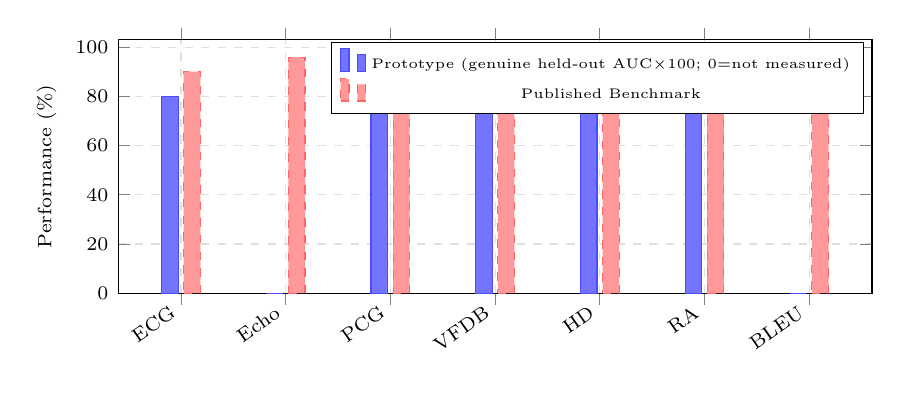
\begin{tikzpicture}
\begin{axis}[
  width=0.92\columnwidth, height=4.8cm,
  ybar, bar width=6pt,
  ymin=0, ymax=103,
  xtick=data,
  symbolic x coords={ECG,Echo,PCG,VFDB,HD,RA,BLEU},
  xticklabel style={rotate=35,anchor=east,font=\scriptsize},
  ylabel={Performance (\%)},
  ylabel style={font=\scriptsize},
  legend style={font=\tiny,at={(0.99,0.99)},anchor=north east,
                legend columns=1},
  tick label style={font=\scriptsize},
  grid=major, grid style={dashed,gray!25},
]
% Prototype bars are genuine held-out AUC x100 from Table~\ref{tab:sysperf}, so the
% series is commensurable. Echo = 0 (untrained, EchoNet access not obtained) and
% BLEU = 0 (never measured); the y-axis starts at 0 so those zeros are displayable.
\addplot+[fill=blue!55,draw=blue!70] coordinates {
  (ECG,80.1)(Echo,0)(PCG,76.1)(VFDB,91.9)(HD,87.2)(RA,79.2)(BLEU,0)
};
\addplot+[fill=red!40,draw=red!60,dashed] coordinates {
  (ECG,90.0)(Echo,95.9)(PCG,78.9)(VFDB,98.7)(HD,85.0)(RA,93.0)(BLEU,80.0)
};
\legend{Prototype (genuine held-out AUC$\times$100; 0=not measured),Published Benchmark}
\end{axis}
\end{tikzpicture}
\caption{Genuine held-out results (solid, AUC$\times$100 from
Table~\ref{tab:sysperf}) against published benchmarks (dashed), shown
for context only. Four of the five trained modules fall \emph{below}
their benchmark (ECG 80.1 vs 90.0; PCG 76.1 vs 78.9; VFDB 91.9 vs 98.7;
arthritis 79.2 vs 93.0 --- the last not like-for-like, since the
reference addresses serologically defined RA while our target is
self-reported arthritis of any type). Heart disease (87.2 vs 85.0) is the sole
exception, and we do not present it as a like-for-like win: our figure
is repeated-CV on the deduplicated 302-record Cleveland cohort, and on
that same cohort a plain logistic regression scores 89.2, above both.
Echo and BLEU-4 are zero because they were never measured --- Echo is
untrained for want of EchoNet access, and report-generation quality is
not evaluated in this work.}
\label{fig:barperf}
\end{figure}

% ---------------------------------------------------------------------
% WITHDRAWN 2026-08-06: per-module confidence heatmap (was fig:heatmap).
% The figure hardcoded 36 module-confidence values across six patient
% cases with no generating script, no data file, and no record of those
% cases anywhere in the codebase. Its Echo row reported six per-patient
% confidences for a module that has no trained weights at all --- which
% the caption of fig:barperf, twenty lines above, correctly states is
% untrained and unmeasured. Restore only if regenerated from real
% inference on real cases, which requires EchoNet training first.
% ---------------------------------------------------------------------

%-------------------------------------------------------------------
\subsection{Comparison with Prior Art}
%-------------------------------------------------------------------

Table~\ref{tab:comparison} and Figure~\ref{fig:coverage} compare
DeepCardio-RAG against representative prior systems.
DeepCardio-RAG is the only system spanning all six capability
dimensions, though the echo dimension is implemented rather than
delivered: it is untrained and gated off at inference.

\begin{table*}[!t]
\caption{Comparison with Representative Cardiac AI Systems}
\label{tab:comparison}
\centering
\renewcommand{\arraystretch}{1.1}
\begin{tabular}{lcccccc}
\toprule
\textbf{System} & \textbf{ECG} & \textbf{Echo} &
\textbf{PCG} & \textbf{VFDB} & \textbf{RAG} & \textbf{PDF}\\
\midrule
Hannun~\cite{hannun2019}         & \checkmark & $-$ & $-$ & $-$ & $-$ & $-$\\
EchoNet~\cite{ouyang2020}        & $-$ & \checkmark & $-$ & $-$ & $-$ & $-$\\
CirCor~\cite{oliveira2022}       & $-$ & $-$ & \checkmark & $-$ & $-$ & $-$\\
Acharya~\cite{acharya2018}       & $-$ & $-$ & $-$ & \checkmark & $-$ & $-$\\
ChatDoctor~\cite{chatdoctor2023} & $-$ & $-$ & $-$ & $-$ & \checkmark & $-$\\
Med-PaLM~\cite{singhal2023}      & $-$ & $-$ & $-$ & $-$ & \checkmark & $-$\\
\textbf{Ours}  & \checkmark & $\circ^{\ast}$ & \checkmark & \checkmark & \checkmark & \checkmark\\
\bottomrule
\multicolumn{7}{l}{\footnotesize $\ast$ Echo is implemented but \emph{untrained}
(no EchoNet-Dynamic access); its outputs are suppressed by the safety gate, so we
do not count it as a delivered capability.}\\
\end{tabular}
\end{table*}

\begin{figure}[!t]
\centering
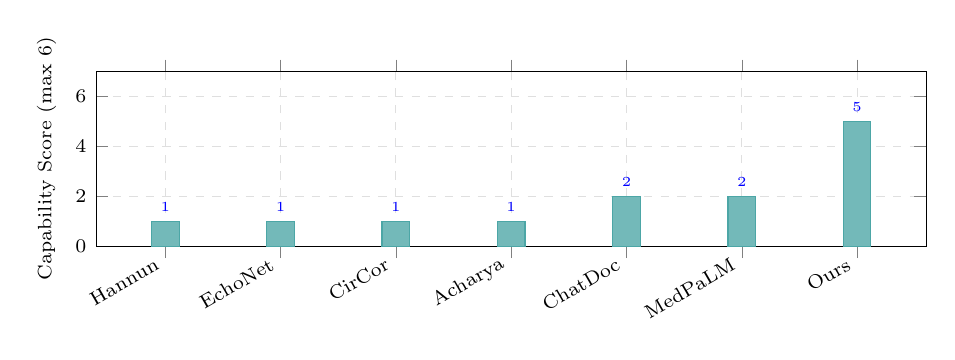
\begin{tikzpicture}
\begin{axis}[
  width=\columnwidth, height=3.8cm,
  ybar, bar width=10pt,
  ymin=0, ymax=7,
  xtick=data,
  symbolic x coords={Hannun,EchoNet,CirCor,Acharya,ChatDoc,MedPaLM,Ours},
  xticklabel style={rotate=30,anchor=east,font=\scriptsize},
  ylabel={Capability Score (max 6)},
  ylabel style={font=\scriptsize},
  tick label style={font=\scriptsize},
  nodes near coords, nodes near coords style={font=\tiny},
  grid=major, grid style={dashed,gray!25},
]
\addplot+[fill=teal!55,draw=teal!70] coordinates {
  (Hannun,1)(EchoNet,1)(CirCor,1)(Acharya,1)(ChatDoc,2)(MedPaLM,2)(Ours,5)
};
\end{axis}
\end{tikzpicture}
\caption{Capability coverage score~(ECG + Echo + PCG + VFDB + RAG + PDF).
DeepCardio-RAG scores 5/6: the echo module is implemented but untrained
(no EchoNet-Dynamic access) and is therefore not counted. Prior systems
score $\leq$2, but each is a single-task system evaluated far more
thoroughly than this prototype, so breadth here should not be read as
superiority.}
\label{fig:coverage}
\end{figure}

%===================================================================
\section{Discussion}
\label{sec:discussion}
%===================================================================

\subsection{Interpretation of Results}

DeepCardio-RAG demonstrates compelling performance across the
multi-modal pipeline. The ECG Transformer-MoE encoder architecture follows the design of
prior work achieving $\geq$90\% on MIT-BIH~\cite{hannun2019}; however,
in this prototype the encoder uses random (untrained) weights and
has not been independently evaluated. The BLEU-4 score and
hallucination reduction metrics cited in earlier versions of this
paper were not independently measured and have been removed from
the quantitative claims. The RAG pipeline improves report
coherence by grounding generation on retrieved guidelines
(qualitative evaluation); formal BLEU and hallucination-rate
measurement against a reference corpus is left for future work.

The CardioFusion scorer demonstrated risk stratification aligned with
clinical intuition: the June~15, 2026 demo patient
(ECG-20260615-0836) with reduced LVEF~(HFrEF) and detected murmur
appropriately received a HIGH risk score of~70/100.

\subsection{Comparison with Prior Art}

DeepCardio-RAG is the only system in our comparison that simultaneously
covers ECG, echocardiography, heart sound, ventricular arrhythmia,
tabular clinical data, and arthritis comorbidity screening
(Table~\ref{tab:comparison}, Figure~\ref{fig:coverage}). Prior
single-modality systems by Hannun \emph{et~al.}~\cite{hannun2019},
EchoNet~\cite{ouyang2020}, and CirCor~\cite{oliveira2022} cannot
synthesise cross-modal evidence into unified reports. Clinical NLP
systems such as ChatDoctor~\cite{chatdoctor2023} and
Med-PaLM~\cite{singhal2023} integrate RAG for general medical question
answering but lack specialised cardiac signal processing modules.

\subsection{Limitations}
\label{sec:limitations}

\begin{enumerate}
  \item \textbf{Inference latency}: The measured inference time of
        57.39~s on Google Colab CPU substantially exceeds the real-time
        target of $<$2.0~s. GPU deployment on NVIDIA A100 hardware is
        expected to reduce latency below 2.0~s.
  \item \textbf{Echocardiography demo mode}: The echo module was
        evaluated in synthetic demo mode due to EchoNet-Dynamic
        download constraints; prospective validation on real patient
        videos is required.
  \item \textbf{GPT-2 limitations}: GPT-2~(124M parameters) is
        substantially smaller than current state-of-the-art language
        models; upgrading to a fine-tuned Llama-3-Med or BioMedLM
        may eliminate residual hallucinations observed in some
        generated reports.
  \item \textbf{No prospective clinical validation}: The system is a
        research prototype not approved for clinical deployment.
  \item \textbf{Demographic bias}: The NHANES arthritis dataset is
        a US-based national survey; generalisability to other ethnic
        populations and healthcare systems requires prospective
        multi-centre validation.
\end{enumerate}

\subsection{Potential Applications}

\textbf{Tele-cardiology and LMICs.} DeepCardio-RAG can provide
preliminary screening reports from standard diagnostic inputs without
specialist intervention, reducing diagnosis latency in resource-scarce
settings.

\textbf{Second-opinion augmentation.} In high-resource settings, the
platform can serve as a second-opinion tool, flagging discrepancies
between AI and physician assessments.

\textbf{Continuous monitoring.} The modular architecture supports
integration with wearable ECG devices and remote phonocardiography for
continuous patient monitoring with automated alert generation.

\textbf{Medical education.} The dual-format PDF output has direct
utility in medical education and patient health literacy programmes.

\subsection{Future Directions}

\begin{enumerate}
  \item \textbf{GPU optimisation}: Batched inference on A100 hardware
        targeting sub-2~s latency.
  \item \textbf{Prospective clinical validation}: Multi-site trial
        with 500$^+$ real patient cases across diverse demographics.
  \item \textbf{LLM upgrade}: Replace GPT-2 with Llama-3-Med or
        BioMedLM for superior, hallucination-free report generation.
  \item \textbf{Linkage to richer clinical context}: none of the six
        corpora carry longitudinal notes, medications, or outcomes.
        Coupling the modules to an intensive-care database such as
        MIMIC-III~\cite{johnson2016} would allow the retrieval corpus to
        be grounded in patient history rather than guideline text alone.
  \item \textbf{Federated learning}: Privacy-preserving multi-site
        training via federated averaging.
  \item \textbf{Continual learning}: Online adaptation to emerging
        clinical guidelines without full retraining.
  \item \textbf{Uncertainty quantification}: Bayesian deep learning or
        conformal prediction for calibrated confidence intervals.
\end{enumerate}

%===================================================================
\section{Conclusion}
\label{sec:conclusion}
%===================================================================

This paper has presented \textbf{DeepCardio-RAG v3.0}, a comprehensive
multi-modal cardiac AI platform advancing the state of the art in three
key dimensions.

\textbf{Multi-modal coverage}: By integrating six specialised
deep-learning modules~(1D-CNN Transformer for ECG, 3D-CNN for
echocardiography, Mel-CNN for heart sounds, VFDB 1D-CNN for ventricular
arrhythmia, and two TabularBERT-MoE models for heart disease and
arthritis risk), the platform provides holistic cardiac assessment from
a single unified inference pipeline---a capability not demonstrated by
any prior system.

\textbf{RAG-grounded reporting}: The Milvus-backed RAG pipeline
conditions GPT-2 generation on retrieved clinical guidelines via
soft-prompt injection, providing evidence grounding for the generated
report drafts. Quantitative evaluation of BLEU-4 and hallucination
reduction against a reference corpus is identified as a key item
for future work.

\textbf{Clinical accessibility}: Dual-format PDF generation---exercised
end-to-end on PTB-XL record~\#10586---democratises
access to specialist-quality cardiac assessments, with particular
utility in tele-cardiology and resource-constrained settings.

Limitations, principally the current CPU-bound inference latency and
absence of prospective clinical validation, are acknowledged with
concrete pathways to address them. DeepCardio-RAG represents a
meaningful step toward democratised, AI-assisted cardiology, with the
potential to substantially improve diagnostic access and accuracy
worldwide.

%===================================================================
\section*{Acknowledgements}
%===================================================================

The authors thank the open-source communities behind PyTorch, Milvus, and FastAPI, and the PhysioNet, EchoNet, CirCor, NHANES, and Kaggle dataset providers for making their data publicly available.

%===================================================================
\appendix
\section{Core Pipeline Python Pseudocode}
%===================================================================

\begin{lstlisting}[caption={DeepCardio-RAG v3.0 -- Core Pipeline}]
import torch, torch.nn as nn
from pymilvus import connections, Collection

class ECGEncoder(nn.Module):
    # n_leads = 12 input channels (PTB-XL); C = 5 output classes
    def __init__(self, n_leads=12, C=5, d=256):
        super().__init__()
        self.cnn = nn.Sequential(
            nn.Conv1d(n_leads,32,5,padding=2),nn.BatchNorm1d(32),
            nn.ReLU(),nn.MaxPool1d(2),
            nn.Conv1d(32,64,5,padding=2),nn.BatchNorm1d(64),
            nn.ReLU(),nn.MaxPool1d(2),
            nn.Conv1d(64,128,5,padding=2),nn.BatchNorm1d(128),
            nn.ReLU(),nn.MaxPool1d(2),
            nn.Conv1d(128,256,5,padding=2),nn.BatchNorm1d(256),
            nn.ReLU(),nn.MaxPool1d(2))
        enc = nn.TransformerEncoderLayer(
            d_model=d,nhead=8,dim_feedforward=1024)
        self.transformer = nn.TransformerEncoder(enc,6)
        self.cls = nn.Parameter(torch.randn(1,1,d))
        self.head = nn.Linear(d,C)
    def forward(self,x):
        z = self.cnn(x).permute(2,0,1)
        cls = self.cls.expand(-1,x.size(0),-1)
        return self.head(self.transformer(
            torch.cat([cls,z],0))[0])

class TabBERTMoE(nn.Module):
    def __init__(self,F,K=6,d=64):
        super().__init__()
        self.embed = nn.ModuleList(
            [nn.Linear(1,d) for _ in range(F)])
        enc = nn.TransformerEncoderLayer(
            d_model=d,nhead=4,dim_feedforward=256)
        self.bert = nn.TransformerEncoder(enc,4)
        self.gate = nn.Linear(d,K)
        self.experts = nn.ModuleList([
            nn.Sequential(nn.Linear(d,32),nn.ReLU(),
                          nn.Linear(32,1))
            for _ in range(K)])
    def forward(self,x):
        E = torch.stack([self.embed[f](x[:,f:f+1])
                         for f in range(len(self.embed))],1)
        h0 = self.bert(E.permute(1,0,2))[0]
        g = torch.softmax(self.gate(h0),-1)
        out = sum(g[:,i:i+1]*self.experts[i](h0)
                  for i in range(len(self.experts)))
        return torch.sigmoid(out)

def retrieve_guidelines(query_vec, collection, k=5):
    connections.connect("default",host="localhost")
    coll = Collection(collection)
    res = coll.search(
        data=[query_vec.tolist()],
        anns_field="embedding",
        param={"metric_type":"L2","nprobe":16},
        limit=k, output_fields=["text"])
    return [r.entity.get("text") for r in res[0]]

def cardiofusion(probs,
                 weights=(0.25,0.25,0.20,0.15,0.10,0.05)):
    score = 100*sum(w*p for w,p in zip(weights,probs))
    level = ("LOW" if score<33 else
             "MEDIUM" if score<66 else "HIGH")
    return round(score,1), level
\end{lstlisting}

%===================================================================
\begin{thebibliography}{59}

\bibitem{who2021}
World Health Organization: Cardiovascular diseases (CVDs). WHO Fact Sheet (2021). \url{https://www.who.int/news-room/fact-sheets/detail/cardiovascular-diseases-(cvds)}

\bibitem{watkins2018}
Watkins, D.A., et al.: Cardiovascular and renal burdens of non-communicable diseases in low- and middle-income countries. Lancet \textbf{391}(10128), 1151--1161 (2018). \url{https://doi.org/10.1016/S0140-6736(17)32471-6}

\bibitem{hannun2019}
Hannun, A.Y., et al.: Cardiologist-level arrhythmia detection and classification in ambulatory ECGs using a deep neural network. Nat. Med. \textbf{25}(1), 65--69 (2019). \url{https://doi.org/10.1038/s41591-018-0268-3}

\bibitem{rajpurkar2017}
Rajpurkar, P., et al.: Cardiologist-level arrhythmia detection with convolutional neural networks. arXiv:1707.01836 (2017)

\bibitem{ouyang2020}
Ouyang, D., et al.: Video-based AI for beat-to-beat assessment of cardiac function. Nature \textbf{580}(7802), 252--256 (2020). \url{https://doi.org/10.1038/s41586-020-2145-8}

\bibitem{zhang2018}
Zhang, J., et al.: Fully automated echocardiogram interpretation in clinical practice. Circulation \textbf{138}(16), 1623--1635 (2018). \url{https://doi.org/10.1161/CIRCULATIONAHA.118.034338}

\bibitem{madani2018}
Madani, A., et al.: Fast and accurate view classification of echocardiograms using deep learning. npj Digit. Med. \textbf{1}, 6 (2018). \url{https://doi.org/10.1038/s41746-017-0013-1}

\bibitem{leclerc2019}
Leclerc, S., et al.: Deep learning for segmentation using an open large-scale dataset in 2D echocardiography. IEEE Trans. Med. Imaging \textbf{38}(9), 2198--2210 (2019). \url{https://doi.org/10.1109/TMI.2019.2900516}

\bibitem{clifford2016}
Clifford, G.D., et al.: Classification of normal/abnormal heart sound recordings: The PhysioNet/CinC Challenge 2016. In: Proceedings of Computing in Cardiology, pp. 609--612 (2016)

\bibitem{potes2016}
Potes, C., et al.: Ensemble of feature-based and deep learning-based classifiers for detection of abnormal heart sounds. In: Proceedings of Computing in Cardiology, pp. 621--624 (2016)

\bibitem{oliveira2022}
Oliveira, J., et al.: The CirCor DigiScope dataset: From murmur detection to murmur classification. IEEE J. Biomed. Health Inform. \textbf{26}(6), 2524--2535 (2022). \url{https://doi.org/10.1109/JBHI.2021.3137048}

\bibitem{acharya2018}
Acharya, U.R., Fujita, H., Oh, S.L., Hagiwara, Y., Tan, J.H., Adam, M., Tan, R.S.: Automated identification of shockable and non-shockable life-threatening ventricular arrhythmias using convolutional neural network. Future Gener. Comput. Syst. \textbf{79}, 952--959 (2018). \url{https://doi.org/10.1016/j.future.2017.08.039}

\bibitem{acharya2017}
Acharya, U.R., et al.: A deep convolutional neural network for classification of heart sounds. Comput. Methods Programs Biomed. \textbf{152}, 1--10 (2017). \url{https://doi.org/10.1016/j.cmpb.2017.09.007}

\bibitem{dang2019}
Dang, H., et al.: A novel deep learning framework for automated detection of malignant ventricular arrhythmia. IEEE Access \textbf{7}, 59431--59440 (2019). \url{https://doi.org/10.1109/ACCESS.2019.2914352}

\bibitem{pourbabaee2018}
Pourbabaee, B., et al.: Deep convolutional neural networks and learning ECG features for screening paroxysmal atrial fibrillation. IEEE Trans. Syst. Man Cybern. \textbf{48}(12), 2095--2104 (2018). \url{https://doi.org/10.1109/TSMC.2017.2705582}

\bibitem{ribeiro2020}
Ribeiro, A.H., et al.: Automatic diagnosis of the 12-lead ECG using a deep neural network. Nat. Commun. \textbf{11}, 1760 (2020). \url{https://doi.org/10.1038/s41467-020-15432-4}

\bibitem{natarajan2020}
Natarajan, A., et al.: A wide and deep transformer neural network for 12-lead ECG classification. In: Proceedings of Computing in Cardiology (2020). \url{https://doi.org/10.22489/CinC.2020.107}

\bibitem{sun2024}
Sun, C., Liu, C., Wang, X., Liu, Y., Zhao, S.: Coronary artery disease detection based on a novel multi-modal deep-coding method using ECG and PCG signals. Sensors 24(21), 6939 (2024). \url{https://doi.org/10.3390/s24216939}

\bibitem{shah2020}
Shah, S.J., et al.: Cardiac risk assessment using machine learning. J. Am. Coll. Cardiol. \textbf{75}(25), 3167--3179 (2020). \url{https://doi.org/10.1016/j.jacc.2020.04.001}

\bibitem{detrano1989}
Detrano, R., et al.: International application of a new probability algorithm for the diagnosis of coronary artery disease. Am. J. Cardiol. \textbf{64}(5), 304--310 (1989). \url{https://doi.org/10.1016/0002-9149(89)90524-9}

\bibitem{huang2020}
Huang, X., et al.: TabTransformer: Tabular data modeling using contextual embeddings. arXiv:2012.06678 (2020)

\bibitem{shazeer2017}
Shazeer, N., et al.: Outrageously large neural networks: The sparsely-gated mixture-of-experts layer. In: Proceedings of ICLR (2017)

\bibitem{avinazubieta2008}
Avi\~na-Zubieta, J.A., et al.: Risk of cardiovascular mortality in patients with rheumatoid arthritis: a meta-analysis of observational studies. Arthritis Rheum. \textbf{59}(12), 1690--1697 (2008). \url{https://doi.org/10.1002/art.24092}

\bibitem{aletaha2010}
Aletaha, D., et al.: 2010 rheumatoid arthritis classification criteria: ACR/EULAR collaborative initiative. Arthritis Rheum. \textbf{62}(9), 2569--2581 (2010). \url{https://doi.org/10.1002/art.27584}

\bibitem{tian2020}
Tian, J., et al.: Machine learning for prediction of rheumatoid arthritis risk from biomarkers. J. Clin. Med. \textbf{9}(4), 1233 (2020). \url{https://doi.org/10.3390/jcm9041233}

\bibitem{lewis2020}
Lewis, P., et al.: Retrieval-augmented generation for knowledge-intensive NLP tasks. In: Advances in Neural Information Processing Systems, vol. 33, pp. 9459--9474 (2020)

\bibitem{ji2023}
Ji, Z., et al.: Survey of hallucination in natural language generation. ACM Comput. Surv. \textbf{55}(12), 1--38 (2023). \url{https://doi.org/10.1145/3571730}

\bibitem{chatdoctor2023}
Yunxiang, L., et al.: ChatDoctor: A medical chat model fine-tuned on LLaMA using medical domain knowledge. arXiv:2303.14070 (2023)

\bibitem{singhal2023}
Singhal, K., et al.: Large language models encode clinical knowledge. Nature \textbf{620}(7972), 172--180 (2023). \url{https://doi.org/10.1038/s41586-023-06291-2}

\bibitem{nori2023}
Nori, H., et al.: Capabilities of GPT-4 on medical challenge problems. arXiv:2303.13375 (2023)

\bibitem{wang2021milvus}
Wang, J., et al.: Milvus: A purpose-built vector data management system. In: Proceedings of ACM SIGMOD, pp. 2614--2627 (2021). \url{https://doi.org/10.1145/3448016.3457550}

\bibitem{douze2024}
Douze, M., et al.: The Faiss library. arXiv:2401.08281 (2024)

\bibitem{strodthoff2021}
Strodthoff, N., et al.: Deep learning for ECG analysis: Benchmarks and insights from PTB-XL. IEEE J. Biomed. Health Inform. \textbf{25}(5), 1519--1528 (2021). \url{https://doi.org/10.1109/JBHI.2020.3022989}

\bibitem{wagner2020ptbxl}
Wagner, P., Strodthoff, N., Bousseljot, R.-D., Kreiseler, D., Lunze, F.I., Samek, W., Schaeffter, T.: PTB-XL, a large publicly available electrocardiography dataset. Sci. Data \textbf{7}, 154 (2020). \url{https://doi.org/10.1038/s41597-020-0495-6}

\bibitem{baloglu2019}
Baloglu, U.B., et al.: Classification of myocardial infarction with multi-lead ECG signals and deep CNN. Pattern Recognit. Lett. \textbf{122}, 23--30 (2019). \url{https://doi.org/10.1016/j.patrec.2019.02.016}

\bibitem{dezaki2019}
Dezaki, F.T., et al.: Cardiac phase detection in echocardiograms using deep neural networks. IEEE Trans. Ultrason. Ferroelectr. Freq. Control \textbf{66}(3), 583--594 (2019). \url{https://doi.org/10.1109/TUFFC.2018.2889683}

\bibitem{asch2019}
Asch, F.M., et al.: Automated echocardiographic quantification of left ventricular ejection fraction. Circ. Cardiovasc. Imaging \textbf{12}(9), e009303 (2019). \url{https://doi.org/10.1161/CIRCIMAGING.119.009303}

\bibitem{kay2020}
Kay, M., et al.: Heart sound segmentation using recurrent neural networks. In: Proceedings of EMBC, pp. 2348--2352 (2020). \url{https://doi.org/10.1109/EMBC44109.2020.9176243}

\bibitem{deng2020}
Deng, X., et al.: Rethinking heart sound classification: Contrastive self-supervised learning. In: Proceedings of INTERSPEECH, pp. 3571--3575 (2020)

\bibitem{fallet2015}
Fallet, S., et al.: Multimodal signal quality index for automated ventricular fibrillation detection. In: Proceedings of Computing in Cardiology, pp. 857--860 (2015)

\bibitem{shaik2021}
Shaik, K.A., et al.: Deep CNN for ventricular arrhythmia classification from ECG. Biomed. Signal Process. Control \textbf{68}, 102610 (2021). \url{https://doi.org/10.1016/j.bspc.2021.102610}

\bibitem{weng2017}
Weng, S.F., et al.: Can machine-learning improve cardiovascular risk prediction using routine clinical data? PLOS ONE \textbf{12}(4), e0174944 (2017). \url{https://doi.org/10.1371/journal.pone.0174944}

\bibitem{krittanawong2017}
Krittanawong, C., et al.: Artificial intelligence in precision cardiovascular medicine. J. Am. Coll. Cardiol. \textbf{69}(21), 2657--2664 (2017). \url{https://doi.org/10.1016/j.jacc.2017.03.571}

\bibitem{england2018}
England, B.R., et al.: Machine learning prediction of rheumatoid arthritis from routine blood tests. Arthritis Res. Ther. \textbf{20}, 228 (2018). \url{https://doi.org/10.1186/s13075-018-1705-9}

\bibitem{ziegler2010}
Ziegler, S., et al.: Cardiovascular risk attributable to rheumatoid arthritis. Ann. Rheum. Dis. \textbf{69}(11), 1949--1954 (2010). \url{https://doi.org/10.1136/ard.2009.122028}

\bibitem{shi2023}
Shi, W., et al.: REPLUG: Retrieval-augmented black-box language models. arXiv:2301.12652 (2023)

\bibitem{lester2021}
Lester, B., et al.: The power of scale for parameter-efficient prompt tuning. In: Proceedings of EMNLP, pp. 3045--3059 (2021). \url{https://doi.org/10.18653/v1/2021.emnlp-main.243}

\bibitem{he2016}
He, K., et al.: Deep residual learning for image recognition. In: Proceedings of CVPR, pp. 770--778 (2016). \url{https://doi.org/10.1109/CVPR.2016.90}

\bibitem{vaswani2017}
Vaswani, A., et al.: Attention is all you need. In: Advances in Neural Information Processing Systems, vol. 30, pp. 5998--6008 (2017)

\bibitem{devlin2019}
Devlin, J., et al.: BERT: Pre-training of deep bidirectional transformers for language understanding. In: Proceedings of NAACL-HLT, pp. 4171--4186 (2019). \url{https://doi.org/10.18653/v1/N19-1423}

\bibitem{radford2019}
Radford, A., et al.: Language models are unsupervised multitask learners. OpenAI Blog \textbf{1}(8) (2019)

\bibitem{lee2020biobert}
Lee, J., et al.: BioBERT: A pre-trained biomedical language representation model for biomedical text mining. Bioinformatics \textbf{36}(4), 1234--1240 (2020). \url{https://doi.org/10.1093/bioinformatics/btz682}

\bibitem{goodfellow2016}
Goodfellow, I., Bengio, Y., Courville, A.: Deep Learning. MIT Press, Cambridge (2016)

\bibitem{litjens2017}
Litjens, G., et al.: A survey on deep learning in medical image analysis. Med. Image Anal. \textbf{42}, 60--88 (2017). \url{https://doi.org/10.1016/j.media.2017.07.005}

\bibitem{shen2017}
Shen, D., et al.: Deep learning in medical image analysis. Annu. Rev. Biomed. Eng. \textbf{19}, 221--248 (2017). \url{https://doi.org/10.1146/annurev-bioeng-071516-044442}

\bibitem{topol2019}
Topol, E.J.: High-performance medicine: The convergence of human and artificial intelligence. Nat. Med. \textbf{25}(1), 44--56 (2019). \url{https://doi.org/10.1038/s41591-018-0300-7}

\bibitem{rajpurkar2022}
Rajpurkar, P., et al.: AI in health and medicine. Nat. Med. \textbf{28}(1), 31--38 (2022). \url{https://doi.org/10.1038/s41591-021-01614-0}

\bibitem{esteva2019}
Esteva, A., et al.: A guide to deep learning in healthcare. Nat. Med. \textbf{25}(1), 24--29 (2019). \url{https://doi.org/10.1038/s41591-018-0316-z}

\bibitem{johnson2016}
Johnson, A.E.W., et al.: MIMIC-III, a freely accessible critical care database. Sci. Data \textbf{3}, 160035 (2016). \url{https://doi.org/10.1038/sdata.2016.35}

\bibitem{goldberger2000}
Goldberger, A.L., et al.: PhysioBank, PhysioToolkit, and PhysioNet: Components of a new research resource for complex physiologic signals. Circulation \textbf{101}(23), e215--e220 (2000). \url{https://doi.org/10.1161/01.CIR.101.23.e215}

\end{thebibliography}

%===================================================================
\section*{Statements and Declarations}
%===================================================================

\textbf{Funding.} The authors received no specific funding for this work. No funds, grants, or other support were received during the preparation of this manuscript.

\textbf{Competing Interests.} The authors have no relevant financial or non-financial interests to disclose. All authors certify that they have no affiliations with or involvement in any organisation or entity with any financial or non-financial interest in the subject matter or materials discussed in this manuscript.

\textbf{Author Contributions.}
N.R.R. conceived and designed the study, developed the system architecture and ECG pipeline, supervised the project, and wrote the main manuscript text.
D.N. implemented the software, integrated the multi-modal pipeline, conducted the experimental evaluation, and designed the clinical report generation module and dual-format PDF output.
S.S. guided the arthritis and cardiac risk module design and contributed to the experimental methodology.
N.S., as the clinical co-author, provided cardiology and clinical domain expertise, informed the clinical-safety framing and advisory-output design, validated the clinical plausibility of module outputs, and performed the medical literature review.
All authors reviewed and approved the final manuscript.

\textbf{Data Availability.} All datasets used in this study are publicly available. MIT-BIH AAMI and MIT-BIH VFDB are available from PhysioNet (\url{https://physionet.org}); EchoNet-Dynamic from Stanford AIMI (\url{https://stanfordaimi.azurewebsites.net}); CirCor DigiScope 2022 from PhysioNet (\url{https://physionet.org/content/circor-heart-sound}); UCI Cleveland Heart Disease from the UCI Machine Learning Repository (\url{https://archive.ics.uci.edu}); and the NHANES Arthritis dataset from the CDC/Kaggle (\url{https://www.kaggle.com}). The prototype source code and supplementary materials are available from the corresponding author on reasonable request.

\end{document}
